\documentclass[journal,letterpaper]{IEEEtran}
\usepackage[letterpaper, left=0.65in, right=0.65in, bottom=0.7in, top=0.7in]{geometry}
\usepackage{stix}
\usepackage{siunitx}
\usepackage[version=4]{mhchem}
\usepackage{booktabs}
\usepackage{makecell}
\usepackage{multirow}
\usepackage{amsmath}
\usepackage{bm}
\usepackage{graphicx}
\usepackage{tikz}
\usepackage{pgfplots}
\usepackage{float}
\usepackage{fancyhdr}
\usepackage[none]{hyphenat}
\usepackage[hidelinks]{hyperref}
\usepackage{import}
\usepackage{transparent}
\usepackage{microtype}

\graphicspath{ {./figures/} }

\pgfplotsset{compat=1.18}

\setlength{\columnsep}{0.2in}
\setlength{\columnwidth}{3.5in}

\newlength\fheight
\newlength\fwidth
\setlength\fwidth{3.25in}
\setlength\fheight{0.8\fwidth}

\newcommand{\incfig}[1]{%
    \centering
    \def\svgwidth{3.5in}
    \import{./figures/}{#1.pdf_tex}
}

\renewcommand{\arraystretch}{1.3}

\sisetup{per-mode = symbol,
         inter-unit-product = \ensuremath{ { } \cdot { } },
         number-unit-product = \text{ },
         group-digits = false,
         detect-weight = true}

\pagestyle{fancy}
\fancyhf{}
\renewcommand{\headrulewidth}{0pt}
\rhead{\thepage}
\lhead{Section 11832 Final Project}

\begin{document}
\title{Effect of Winglet Cant Angle on Lift-to-Drag Ratio}

\author{\IEEEauthorblockN{\LARGE{Borg, Auston J. \quad Lam, Brandon H. \quad Latzko, Alexander J. \\}}
\IEEEauthorblockA{
Section 11832 \quad December 6, 2023}
}

\maketitle
\thispagestyle{empty}

\begin{abstract}
This study examines the relationship between the cant angle of a winglet and the lift-to-drag ratio of the airfoil section by using a calibrated dynamometer.
The main objective of this experiment was to create a model for the relationship between the cant angle and the lift-to-drag ratio, $\bm{L/D}$.
A secondary objective was to determine if adjusting the cant angle could lead to an optimal angle for maximizing the lift-to-drag ratio of the airfoil section.
Winglets disrupt the formation of wingtip vortices and force the airflow to become more two-dimensional, reducing the induced drag of the wing.
Unlike other wing features such as flaps and ailerons, winglets cannot be adjusted during flight to provide the most optimal setting for the aircraft.
The theory behind this experiment is that by adjusting the cant angle, the most optimal performance during simulated cruise conditions can be achieved.
It was found that the optimal cant angle for the performance of the wing was $\bm{42 \pm }\ang{1}$.
The relative difference between theoretical data obtained using XFLR5 and the experimental data ranged from 6.4\% to 14.1\% for the values of the lift-to-drag ratio.
This was caused by the surface roughness of the 3D printed wing section and the mounting equipment used to attach it to the dynamometer.
The results showed that the lift-to-drag ratio slightly increased with the cant angle until reaching its optimal value, after which the parasitic drag caused by the attachment causes the ratio to decline in magnitude.
\end{abstract}

\begin{IEEEkeywords}
cant angle, lift-to-drag ratio, winglet, XFLR5
\end{IEEEkeywords}


\section{Introduction}


\IEEEPARstart{I}{n} the field of commercial aviation, more than 45,000 planes take off each day~\cite{FAA}.
To reduce costs and promote more sustainable flights, airlines have consistently sought out ways to enhance the efficiency of their aircraft.
One important measure of an aircraft's efficiency is its lift-to-drag ratio.
A high lift-to-drag ratio allows an aircraft to carry larger payloads while requiring less thrust to overcome drag.
One technique used in modern aircraft is the addition of winglets to the tips of the wings.
These winglets disrupt the wingtip vortices and force the airflow to become more two-dimensional, reducing the induced drag on the wing~\cite{NASA}.
Despite their use in the aviation industry for many years, there is a surprising lack of publications providing specific details on efficient winglet design.
One consideration in winglet design is the winglet cant angle, which is the angle that the winglet makes with the span of the wing, as shown in Fig.~\ref{fig:cant}.

\begin{figure}[H]
    \centering
    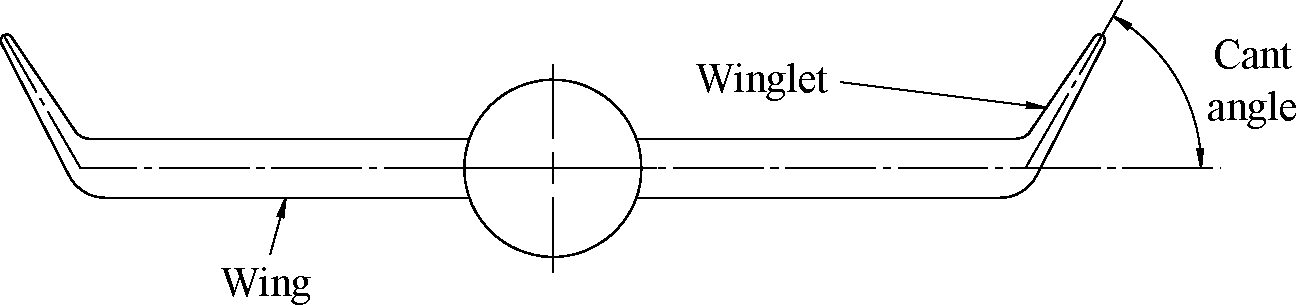
\includegraphics[width=3.45in]{cantDiag}
    \caption{A simplified diagram that illustrates how the cant angle relates the orientation of the winglet to the span of the wing~\cite{cantDiag}.}
    \label{fig:cant}
\end{figure}
\noindent
Previous research has suggested that the lift-to-drag ratio generally increases with the cant angle.
However, once the cant angle passes a certain point, the increase in friction drag begins to decrease the aerodynamic efficiency~\cite{variableCant}.

The experiment involved creating 3D printed wings with interchangeable winglets.
These winglets had varying cant angles, ranging from 0 to 90 degrees.
Fig.~\ref{fig:wing} shows an example of one of these wings.
\begin{figure}[H]
    \centering
    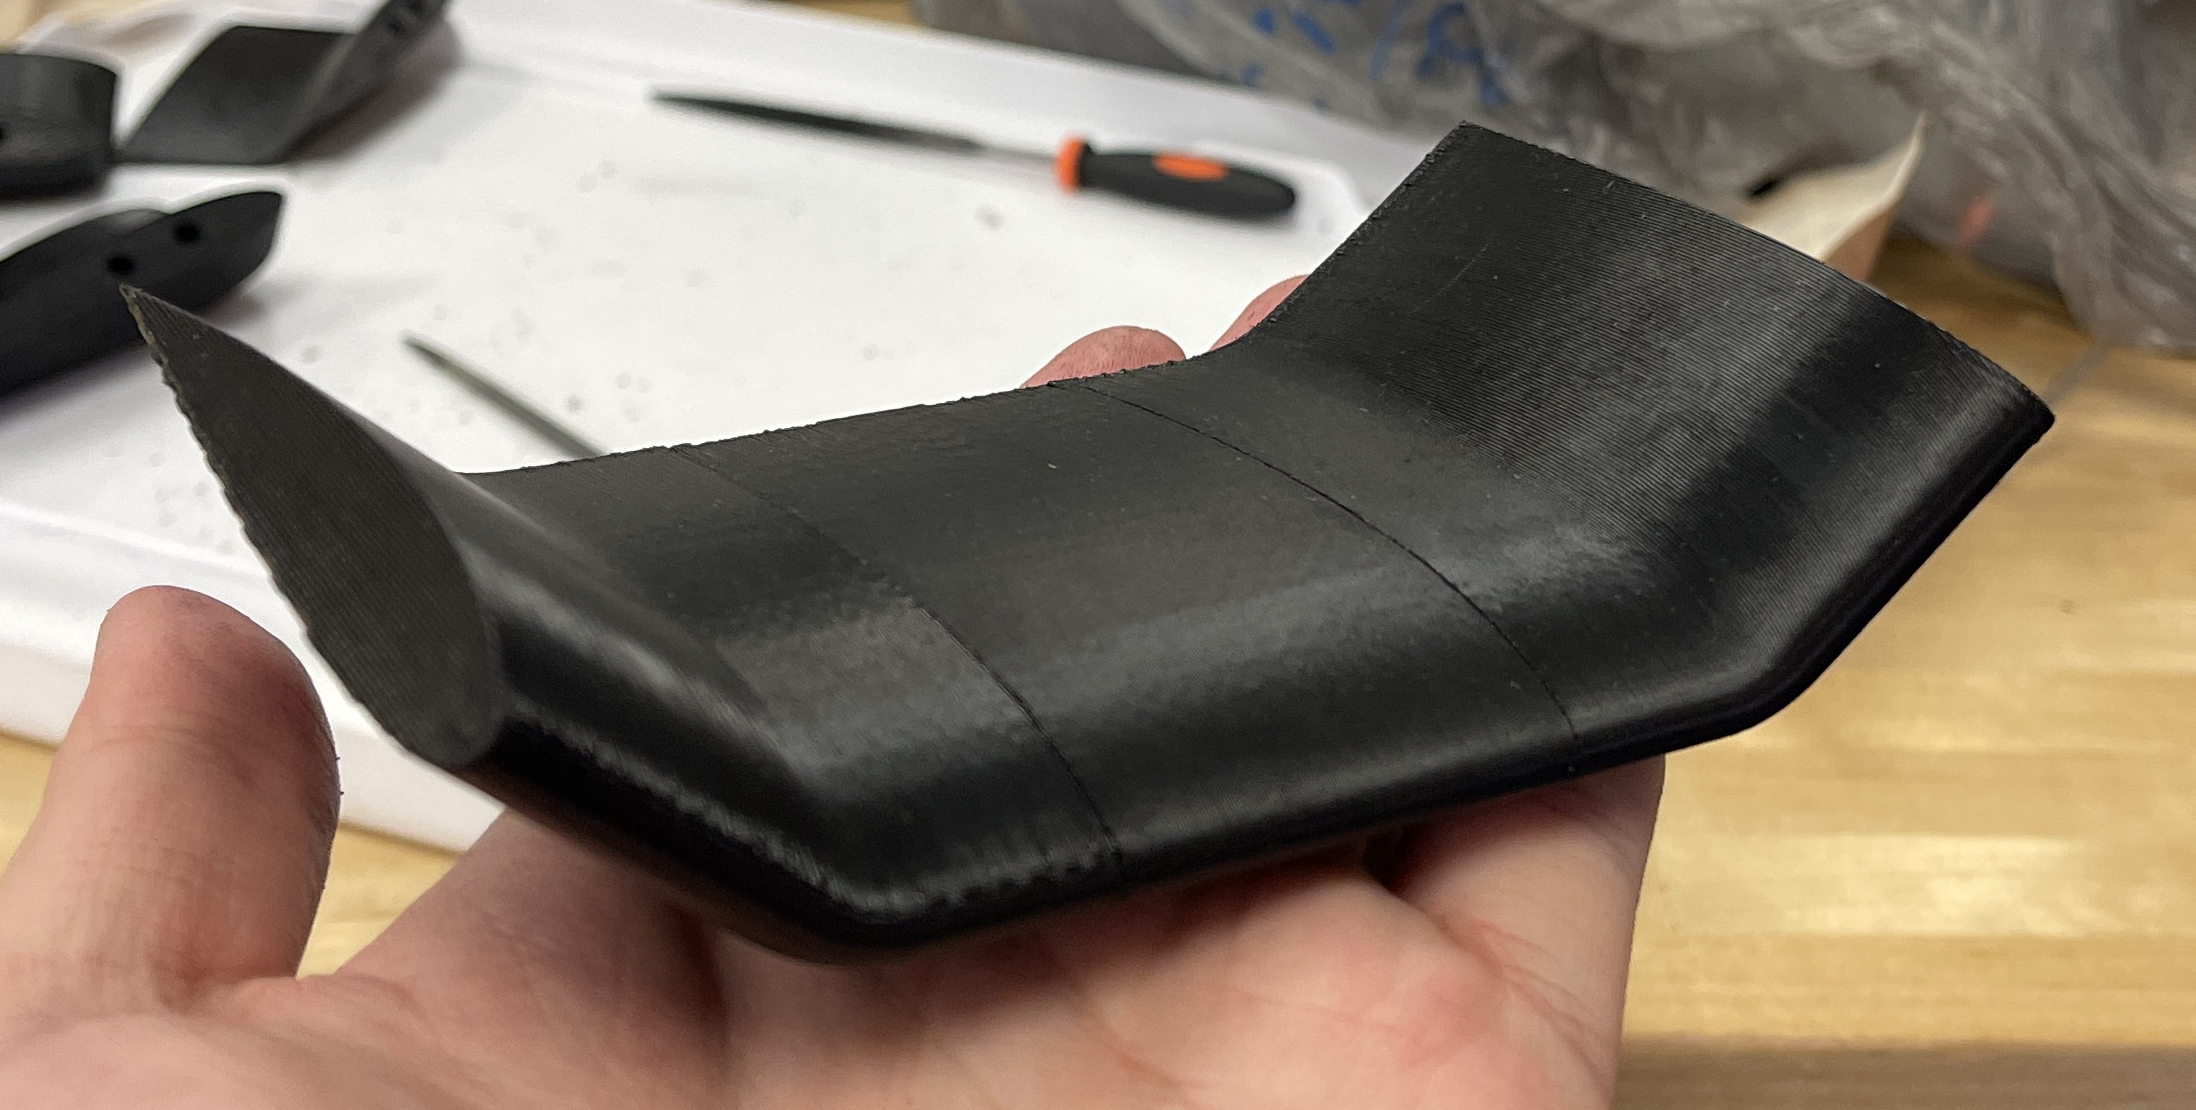
\includegraphics[width=3.5in]{wing}
    \caption{A 3D printed model of the wing used in the experiment. The specific configuration shown has a cant angle of \ang{40}.}
    \label{fig:wing}
\end{figure}
\noindent
The wind tunnel was adjusted to a desired Reynolds number of 100,000 by using the tunnel calibration coefficient determined previously~\cite{lab1}.
The desired drop in static pressure was related to the Reynolds number using~\eqref{eq:eq1}, where $K$ is the tunnel calibration coefficient, $\nu$ is the dynamic viscosity of air, $\rho$ is the density of the air, $c$ is the chord length of the airfoil, and $Re$ is the desired Reynolds number.
\begin{equation} \label{eq:eq1}
    \Delta P = \frac{\frac{1}{2}\rho (1 - K)\nu^2}{c^2} {Re}^2
\end{equation}

The objectives of this experiment included first characterizing the relationship between the winglet cant angle and the lift-to-drag ratio of a wing by determining an equation that properly represents the experimental data.
The second objective was to use this equation to determine the optimal cant angle that maximizes the lift-to-drag ratio.
Finally, the software XFLR5 was also used to compare theoretical data to experimental data.


\section{Procedure}

\subsection{Manufacturing of the Wing}

The wing was 3D printed using a fused deposition modeling (FDM) printer in ASA thermoplastic.
The model for the 3D print was created using the CAD software SolidWorks.
It was divided into three sections, consisting of the wing base and two winglets.
The selected airfoil was the NACA2415, and the wing was set at an angle of attack of 10 degrees.
This angle of attack was selected to ensure that a non-negligible lift force would be generated by the airfoil.
The wing base was designed with two hexagonal pins on each side, which were intended to press fit into the corresponding holes on the winglet pieces, as depicted in Fig.~\ref{fig:Airfoil}.

\begin{figure}[H]
    \centering
    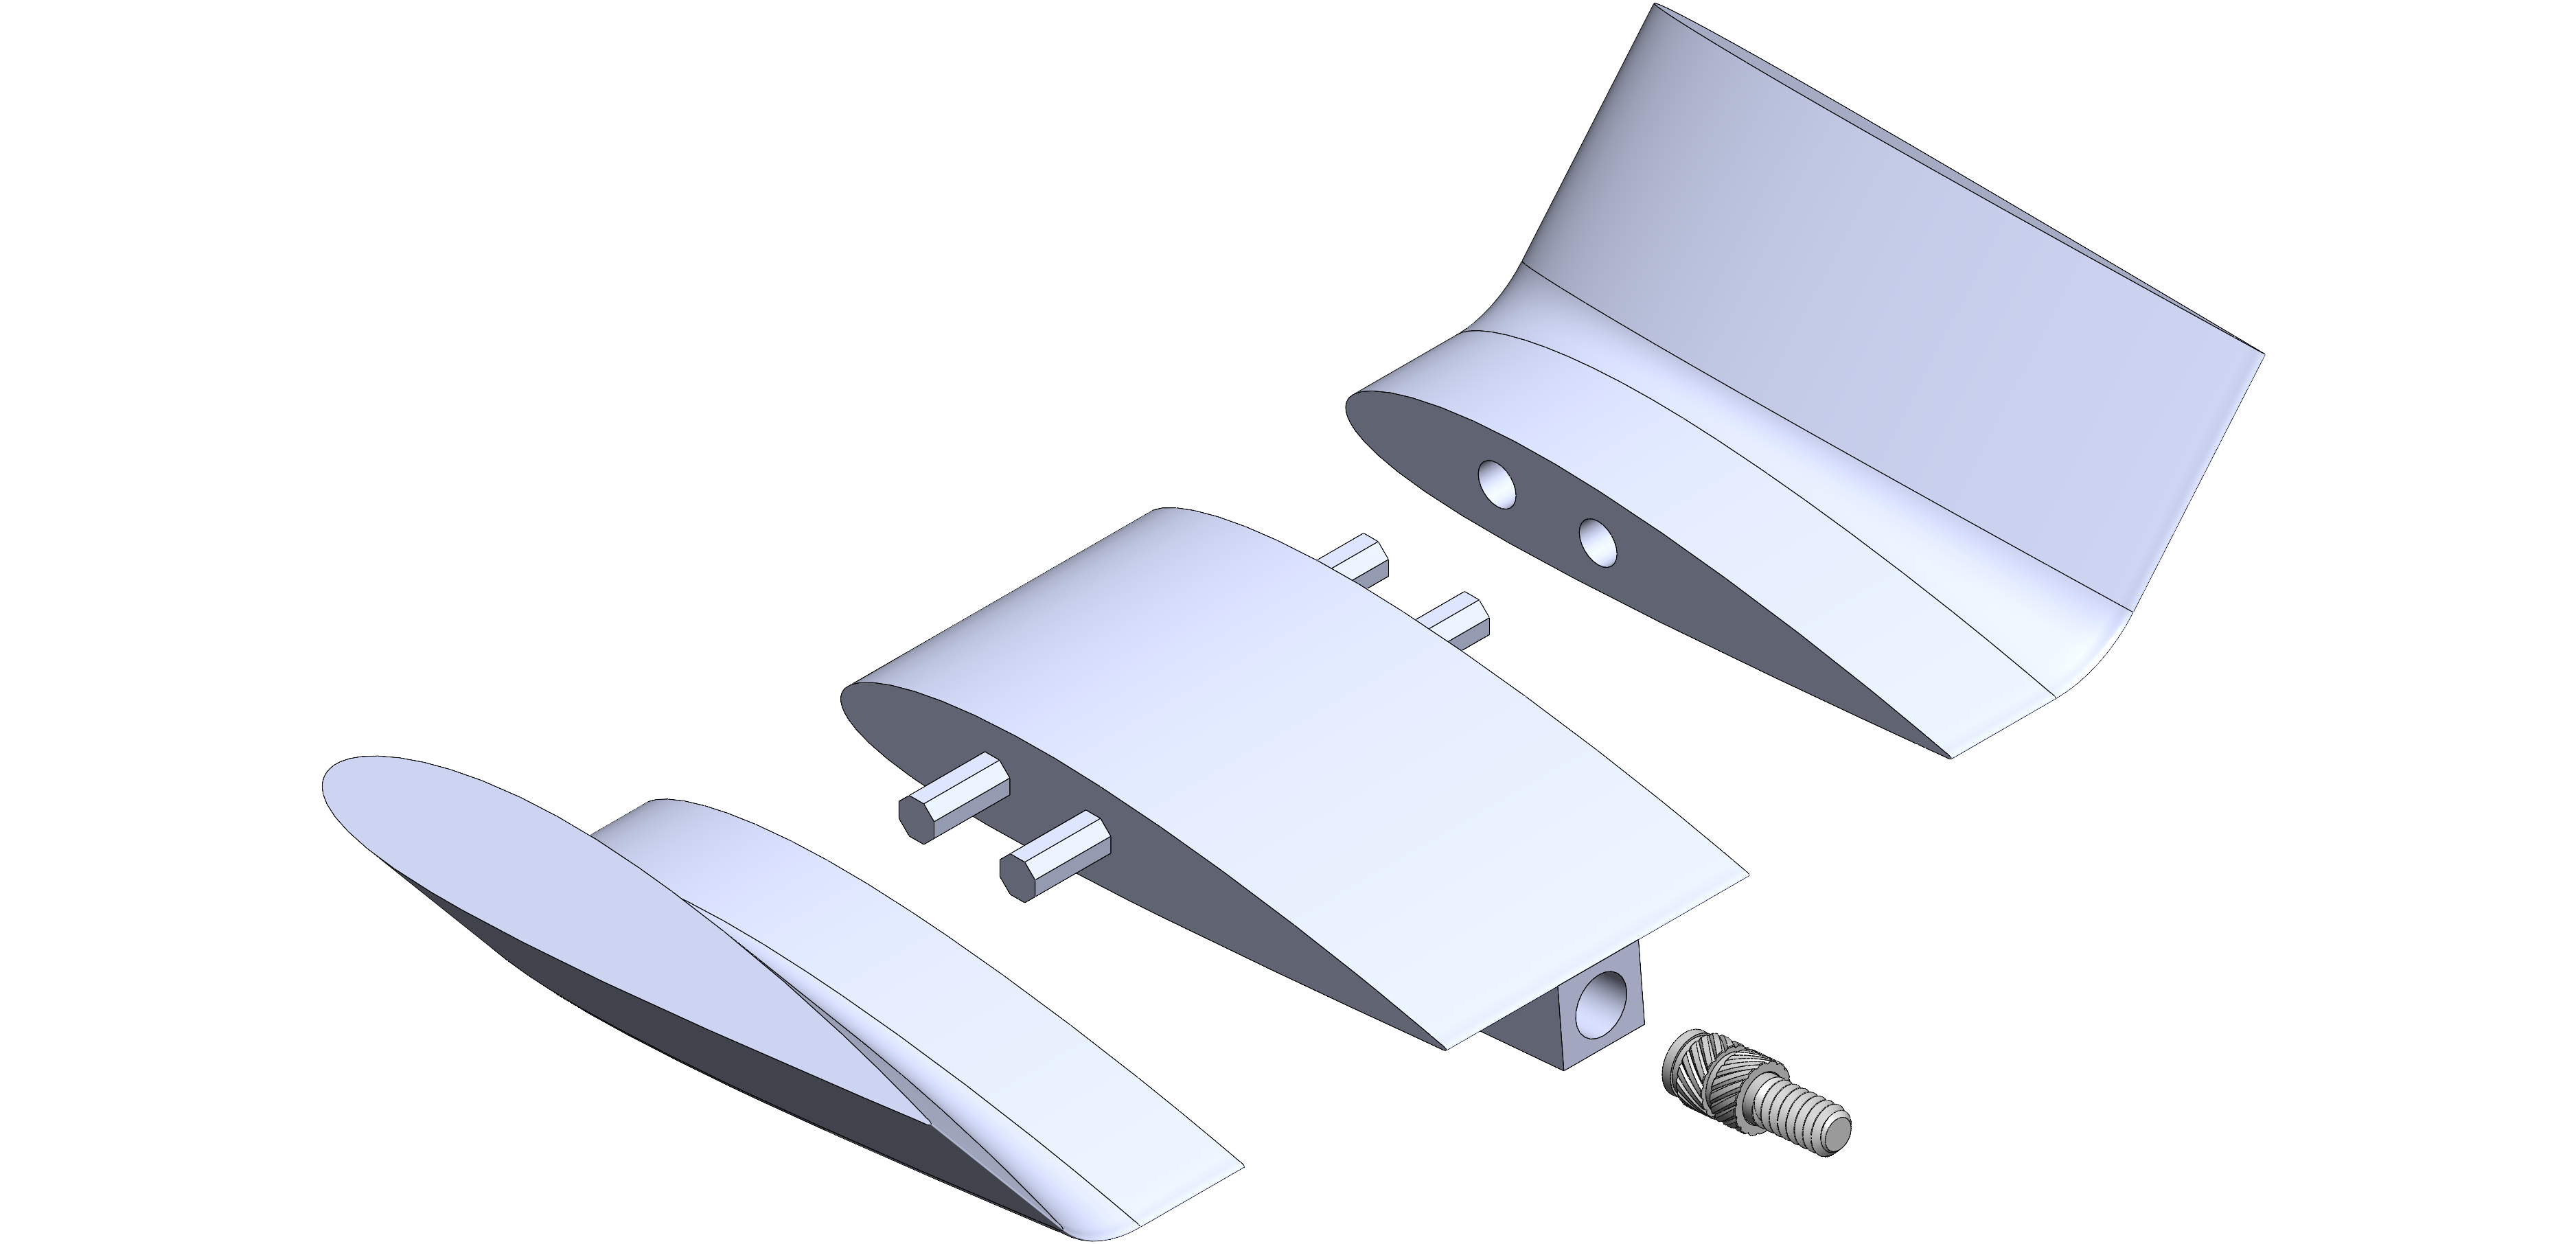
\includegraphics[width=3.5in]{Airfoil}
    \caption{SolidWorks 3D model of the wing section used in this experiment. The specific configuration shown has a cant angle of \ang{50}.}
    \label{fig:Airfoil}
\end{figure}

The winglet pieces had ten different configurations with cant angles ranging from 0 to 90 degrees.
Each configuration maintained a constant wingspan to ensure consistency across trials.
A total of twenty winglet pieces were manufactured, with ten for each side of the wing.
The chord length of the airfoil was $76.2 \pm \qty{0.2}{\mm}$, and the wingspan of the airfoil section was $139.8 \pm \qty{0.2}{\mm}$, as measured with calipers.
A 10-24 male heat-set insert was mounted onto the wing base to allow for proper threading of the wing into the 10-24 threaded hole in the dynamometer.

\subsection{Calibration of the Dynamometer}

For this experiment, the dynamometer was calibrated for both lift and drag.
To perform the calibration, metal weights were weighed using a scale.
Once the weights were recorded, they were placed on the dynamometer, which was set up in a configuration such that the weight would be loaded perpendicular to the length of the stand for drag calculation, as shown in Fig.~\ref{fig:drag}.

\begin{figure}[H]
    \centering
    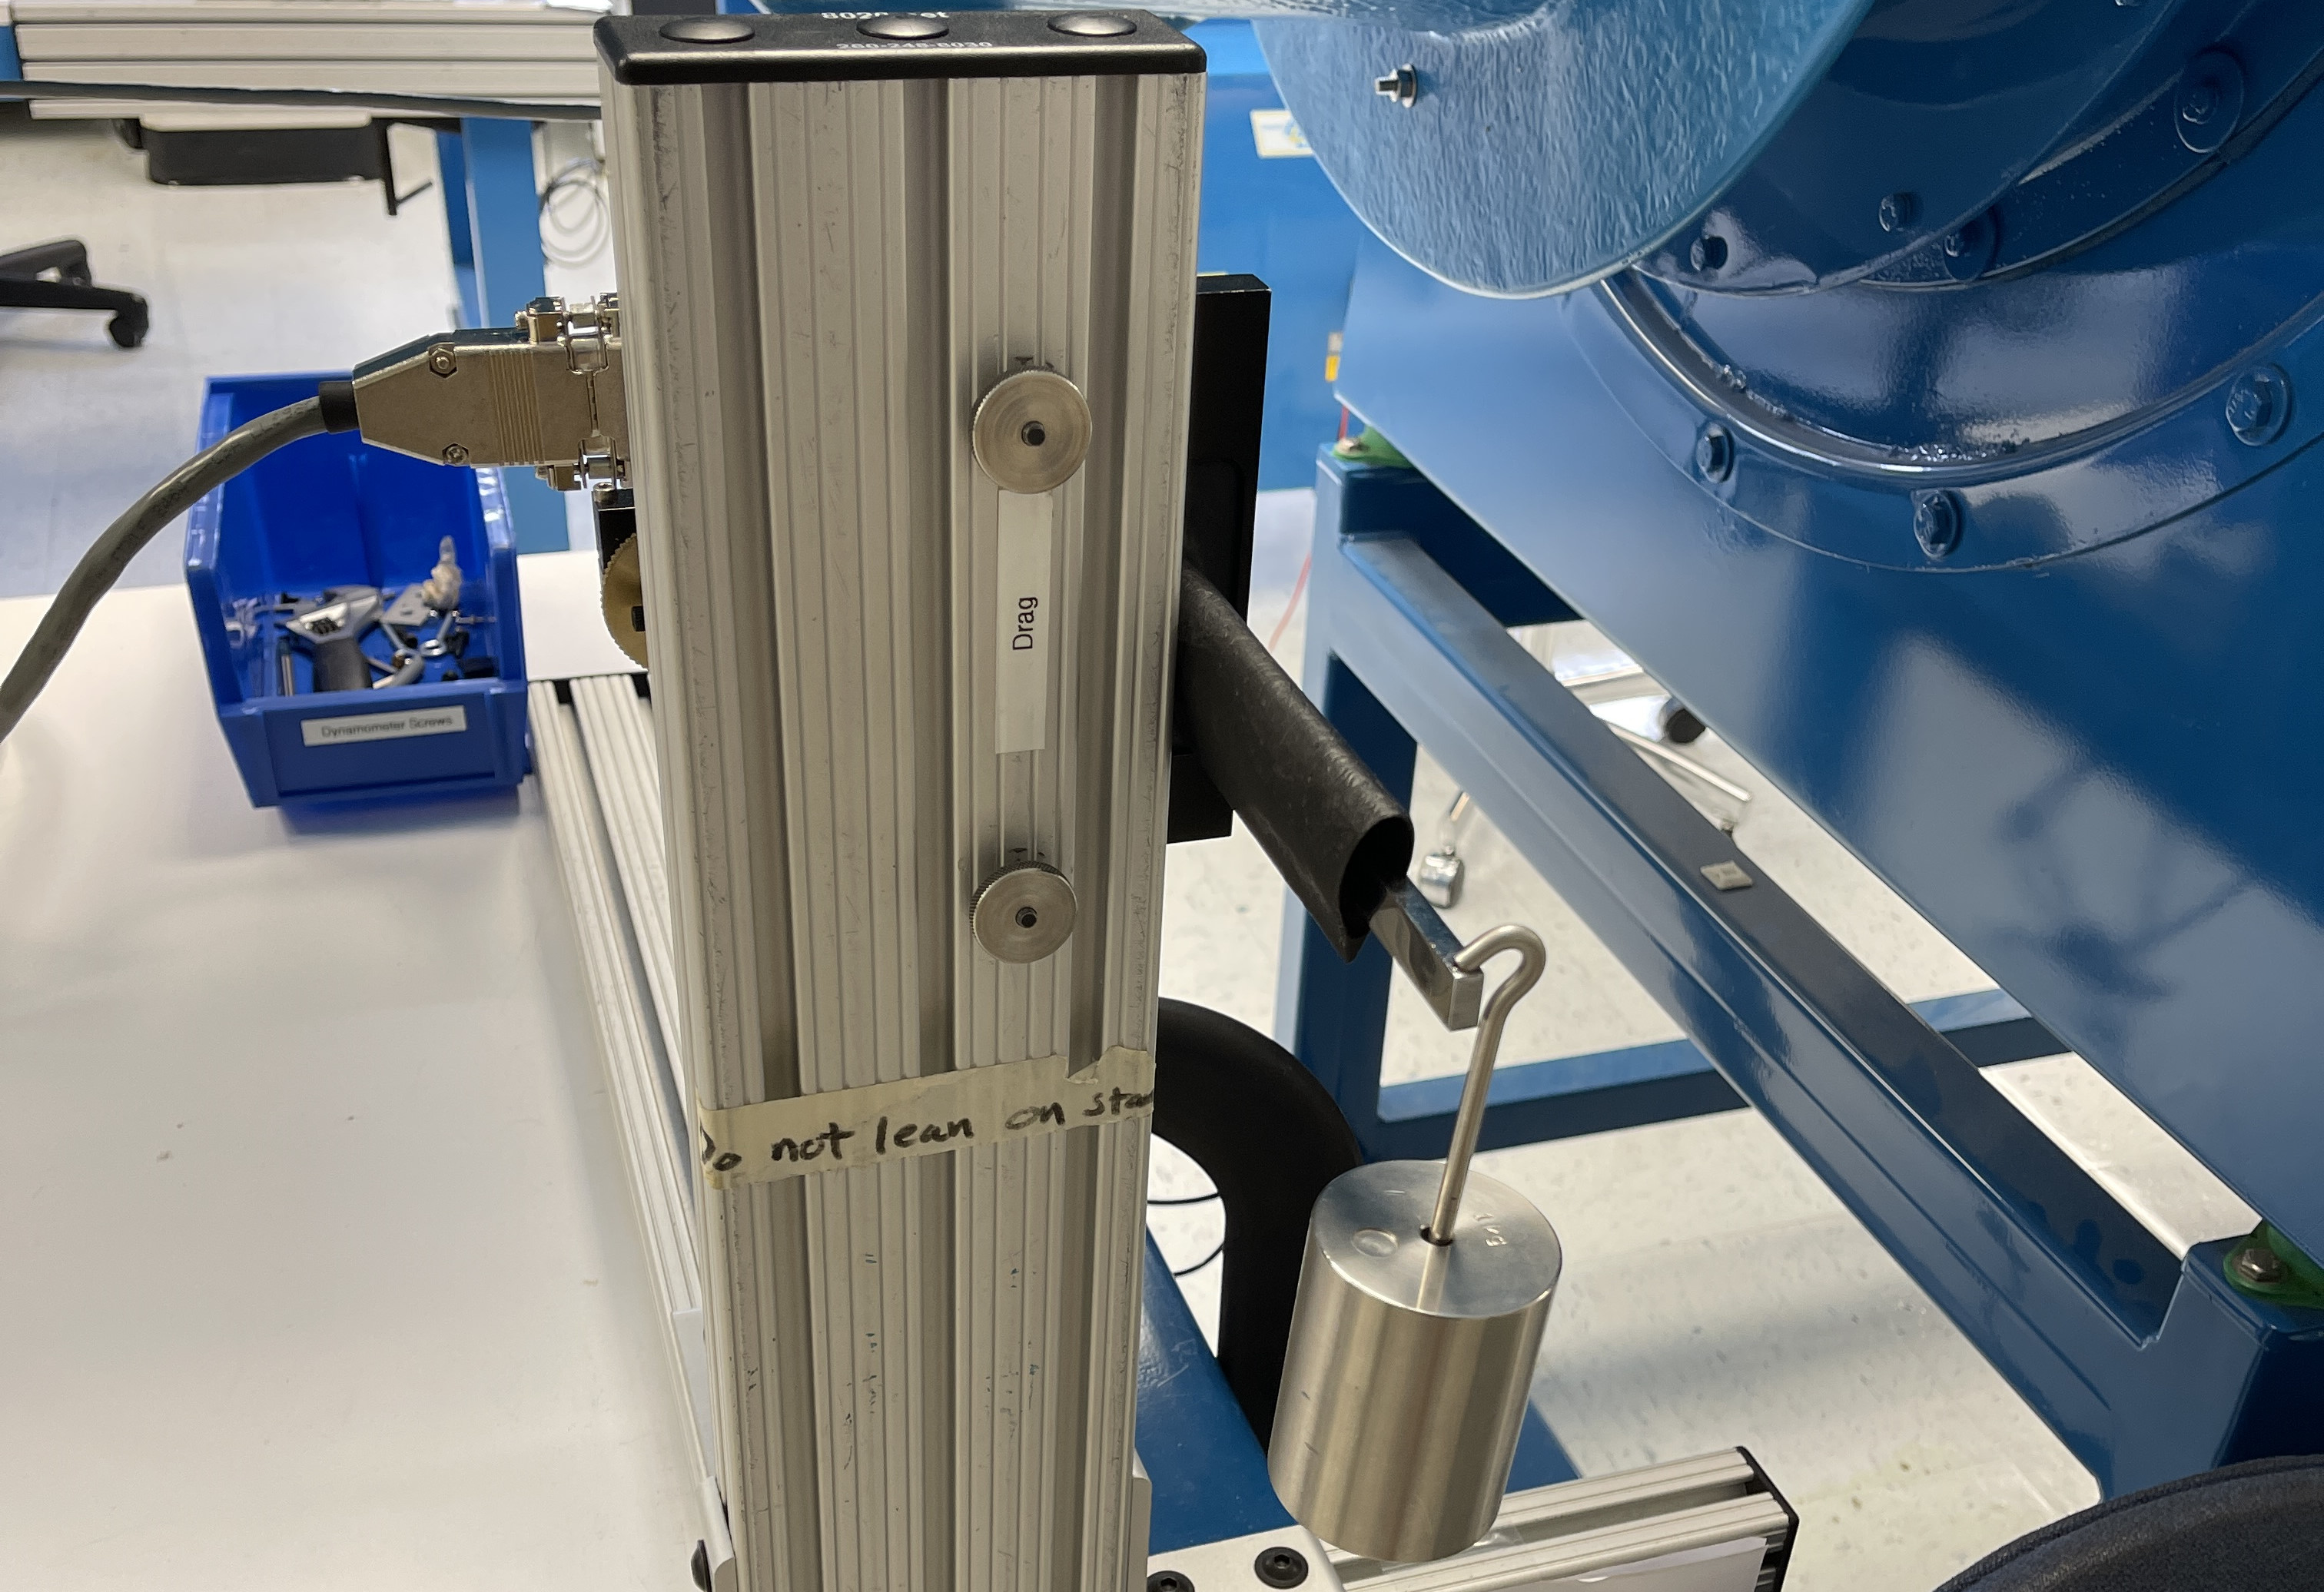
\includegraphics[width=3.5in]{drag}
    \caption{Dynamometer setup for calibrating the drag calculation with a \qty{500}{\g} weight loaded.}
    \label{fig:drag}
\end{figure}

A total of twelve different mass configurations were measured, ranging from \qty{0.000}{\kg} to \qty{2.270}{\kg}.
The maximum mass corresponds to the maximum force that the dynamometer can measure.
The weights were attached to the dynamometer using a hook attached to the weight itself.
Additional weights needed to reach the desired weight were attached to the bottom of each weight using the hook.

To zero the drag force, the drag LVDT wheel was adjusted until the voltage display read zero when no weight was loaded.
Then, the maximum weight was placed on the dynamometer and the gain potentiometer was adjusted until a voltage of \qty{-10}{\V} was displayed.
The weights were then removed, and the display was verified to show zero voltage.
This process was repeated for each weight configuration.

The same procedure was performed for the lift calibration, except this time the desired maximum voltage for the zero verification was \qty{10}{\V}.
The dynamometer was also reoriented so that the weights acted parallel to the length of the dynamometer, in the lift direction by threading an eyebolt, as shown in Fig.~\ref{fig:lift}.
The slope of the line obtained from both calibrations was then used to determine force values for the experiment.

\begin{figure}[H]
    \centering
    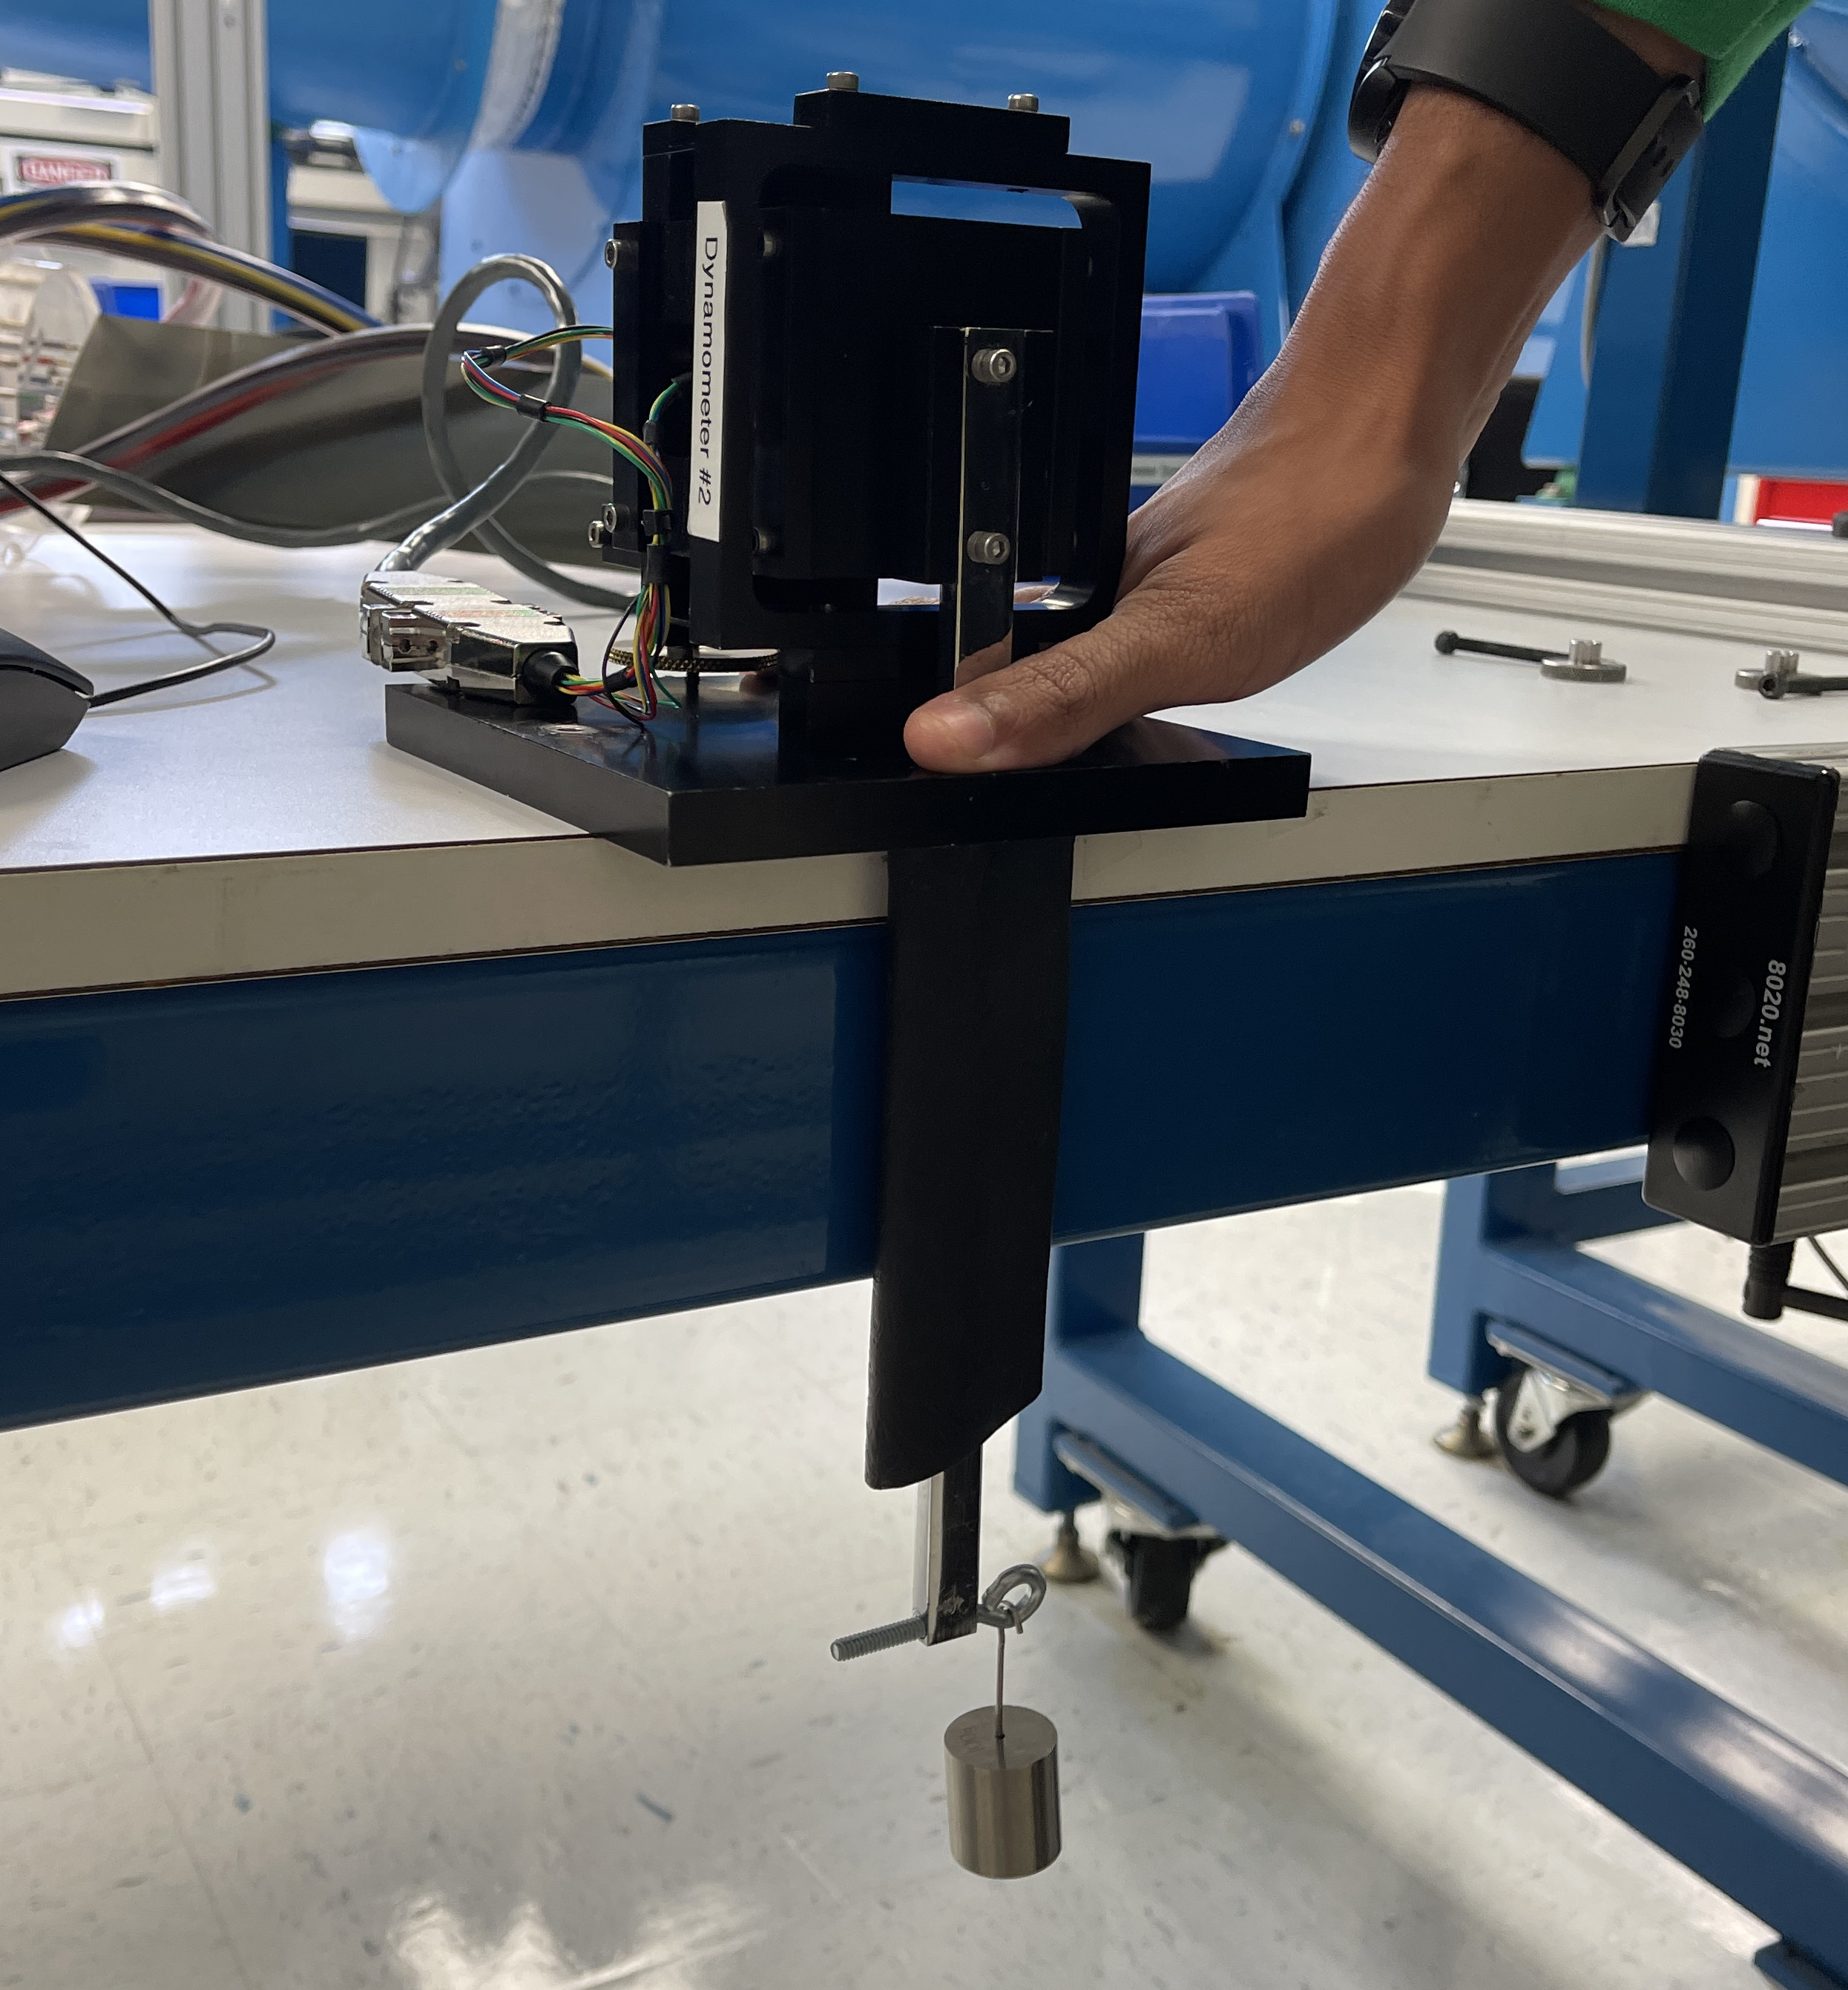
\includegraphics[width=3.5in]{lift}
    \caption{Dynamometer setup for calibrating the lift calculation with a \qty{200}{\g} weight loaded.}
    \label{fig:lift}
\end{figure}

\subsection{Measuring Lift and Drag}

The ambient pressure, relative humidity, and ambient temperature were recorded.
To measure the air velocity in the wind tunnel, the pressure transducer was calibrated in inches of water in the negative direction using the digital readout on the transducer and a water manometer.
The desired Reynolds number for this experiment was 100,000 to simulate cruise conditions for an RC aircraft with the same chord length.
To achieve this, the wind tunnel speed was adjusted until the pressure readout matched the desired static gauge pressure for the current ambient conditions.
The zero drag and lift weight of the dynamometer were then recorded by placing the dynamometer in the wind tunnel and recording the voltages displayed on the pressure transducer.
The wing base section was positioned in the test section by using the 10-24 male heat-set insert located at the back of the central span.
Next, the appropriate winglet pieces with the specific cant angle were attached to the wing base, as shown in Fig.~\ref{fig:wingInside}.
\begin{figure}[H]
    \centering
    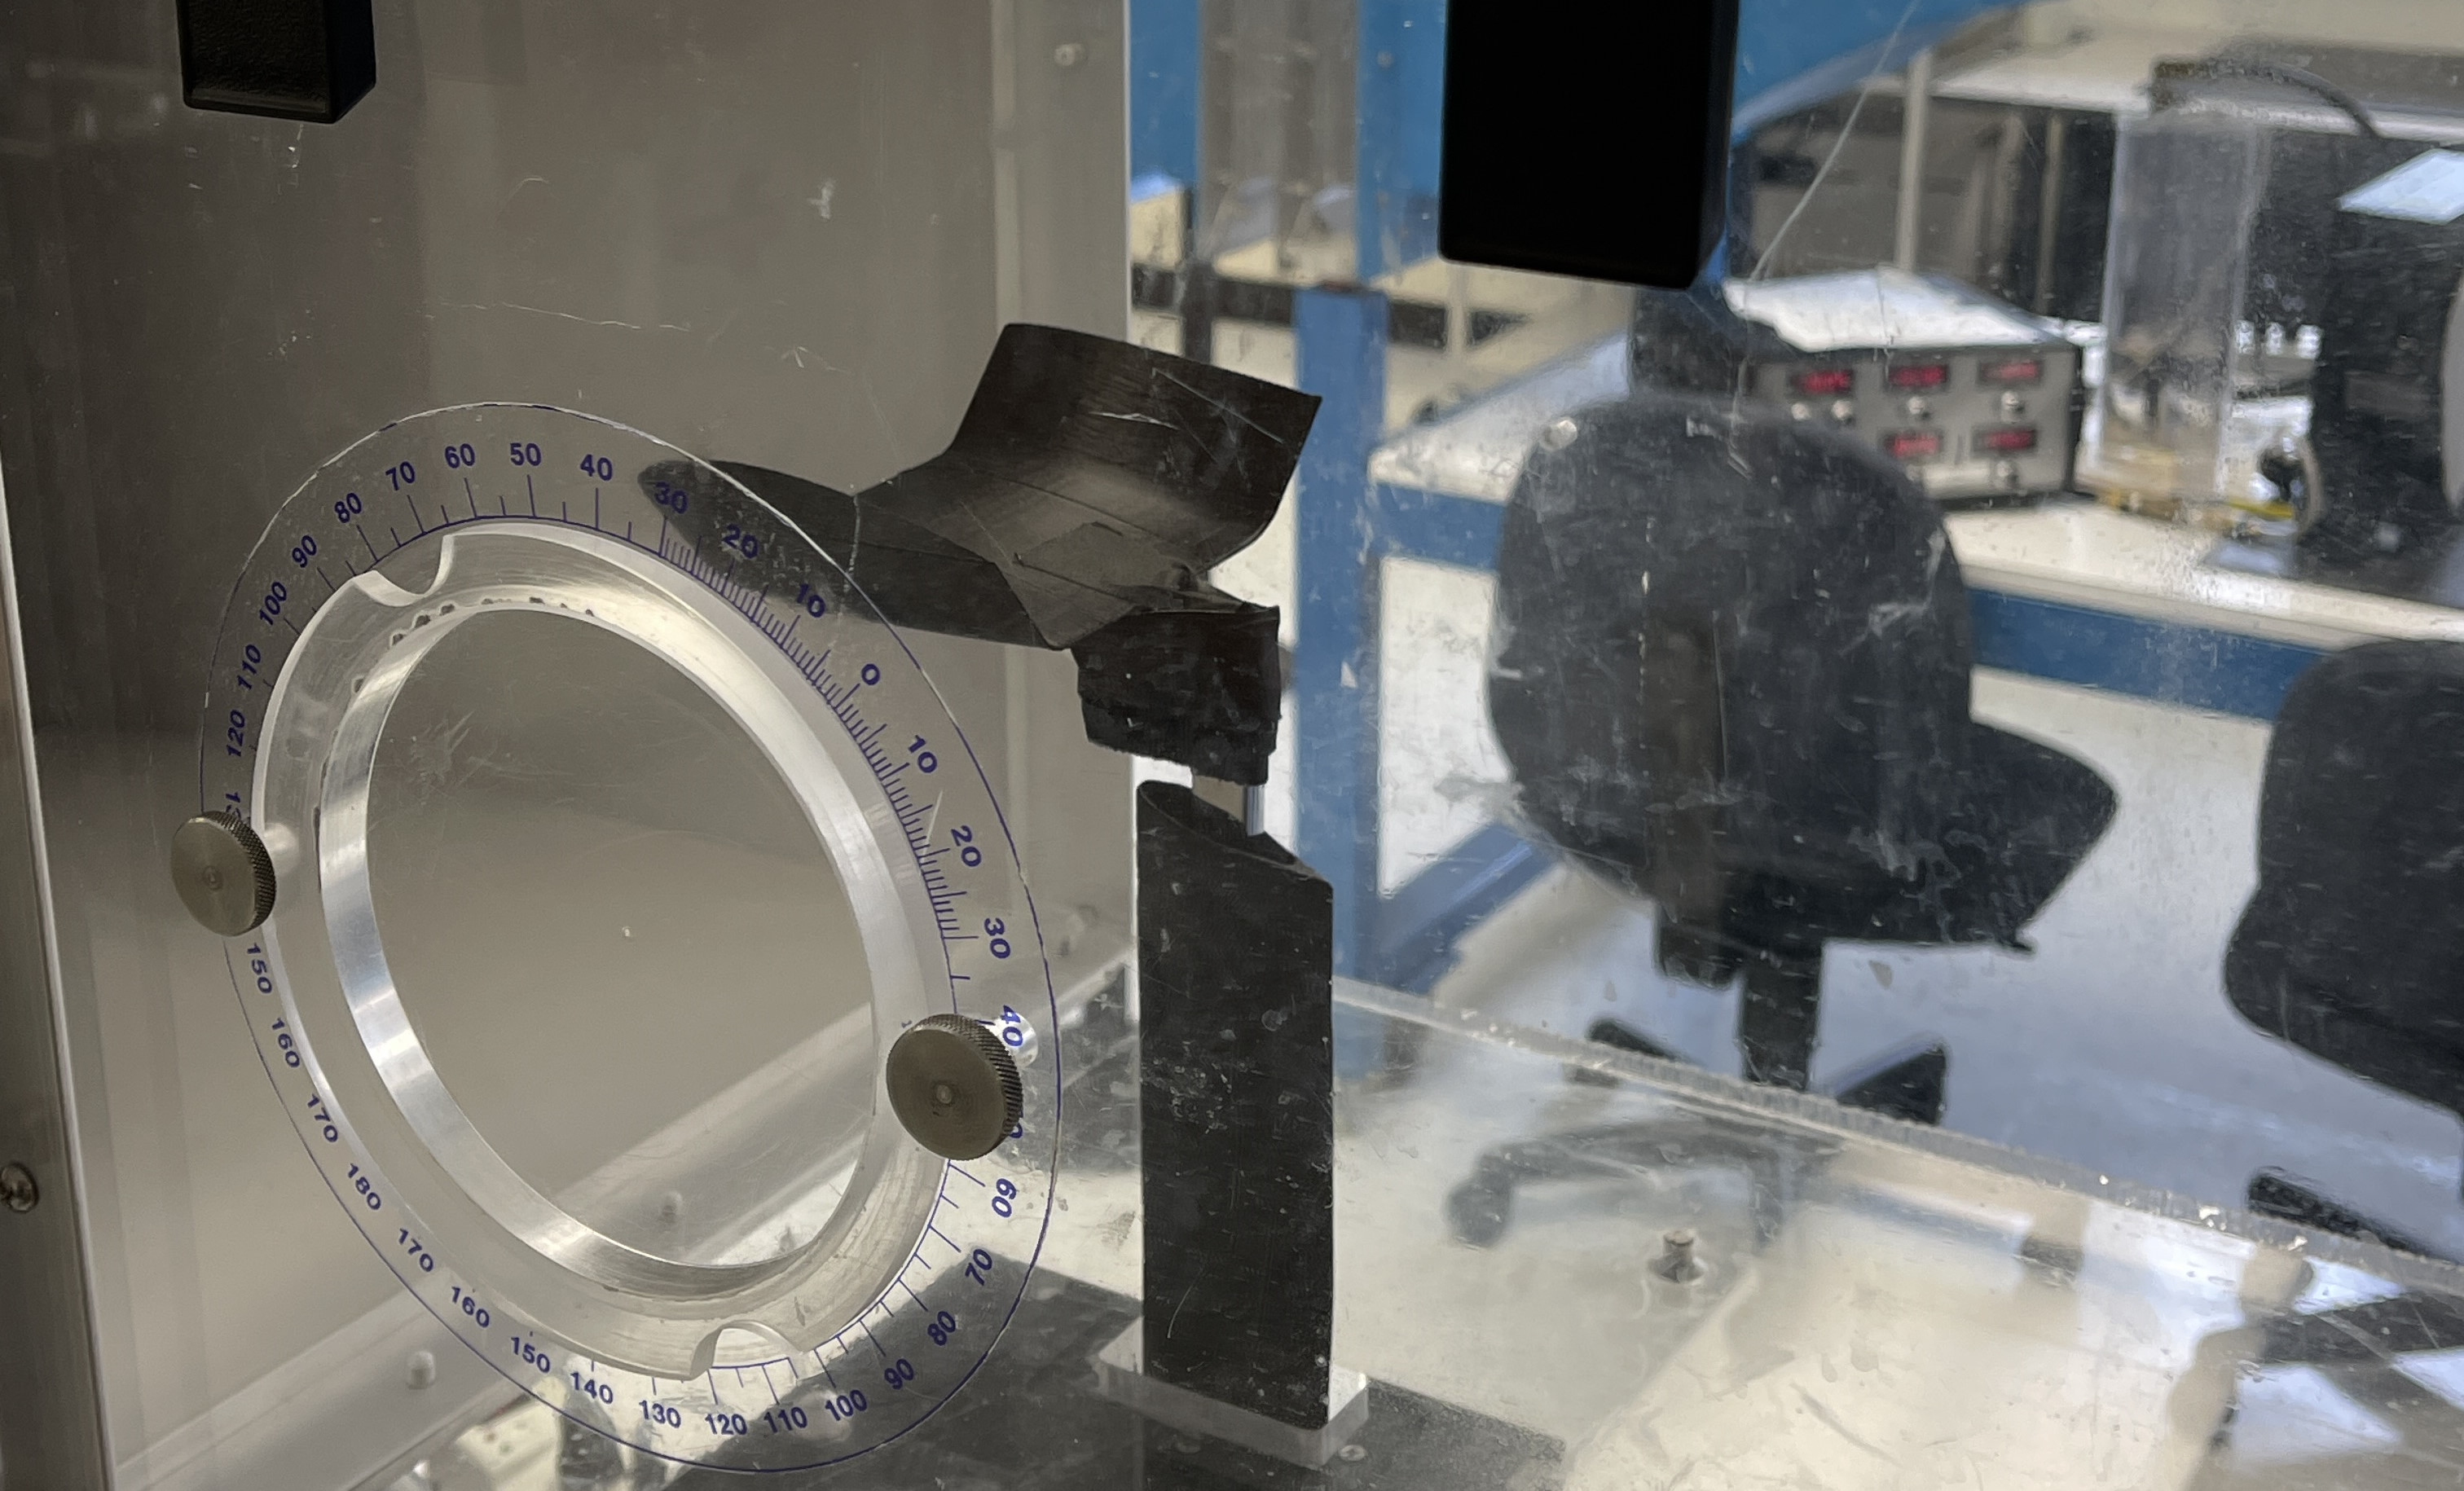
\includegraphics[width=3.5in]{wingInside}
    \caption{Wing section with the \ang{40} winglets inside the test section of the wind tunnel.}
    \label{fig:wingInside}
\end{figure}
\noindent
The wind tunnel was set to the previously determined speed to ensure the correct Reynolds number was achieved.
The lift and drag voltages were recorded, with care taken to tare out the zero lift and drag voltages.
This process was repeated for each of the remaining cant angles.

\subsection{XFLR5 Simulation}

The wing was replicated in XFLR5 using the integrated plane design tool.
The cant angle of the airfoil section was adjusted in XFLR5 using the dihedral angle option in the wing design section.
The analysis method employed was the ring vortex method, with an airspeed of \qty{20}{\m\per\s}.
The simulation was performed at an angle of attack of 10 degrees, to replicate the experimental setup.
The coefficients of lift and drag were recorded for each cant angle during the simulation.


\section{Results}


The ambient pressure, $P_\text{amb}$, of the room was measured using a wall-mounted barometer.
The temperature, $T$, and the relative humidity, $\varphi$, of the room was measured using a digital thermometer and hygrometer placed next to the test section.
The measured atmospheric conditions are summarized in Table~\ref{tab:atmCond}.

\begin{table}[H]
    \centering
    \caption{Atmospheric Conditions}
    \renewcommand{\arraystretch}{1.4}
    \begin{tabular}{ccc}
    \toprule
    Parameter & Value & Uncertainty ($\pm$) \\ \midrule \midrule
    $P_\text{amb}$ & \qty{764.10}{mm\ce{Hg}} & \qty{0.02}{mm\ce{Hg}} \\
    $T$ & \qty{22.9}{\celsius} & \qty{0.1}{\celsius} \\
    $\varphi$ & 40\% & 1\% \\ \bottomrule
    \end{tabular}
    \label{tab:atmCond}
\end{table}

To calibrate the dynamometer for lift and drag force measurements, twelve different mass configurations were used.
These masses were loaded on the dynamometer in both its drag and lift configurations, as shown in Fig.~\ref{fig:drag} and \ref{fig:lift}, respectively.
The masses were then converted into weights and plotted against their corresponding voltages for lift and drag as illustrated in Fig.~\ref{fig:calL} and \ref{fig:calD}, respectively.

\begin{figure}[H]
    \centering
    % This file was created by matlab2tikz.
%
%The latest updates can be retrieved from
%  http://www.mathworks.com/matlabcentral/fileexchange/22022-matlab2tikz-matlab2tikz
%where you can also make suggestions and rate matlab2tikz.
%
\definecolor{mycolor1}{rgb}{0.65098,0.65098,0.65098}%
%
\begin{tikzpicture}

\begin{axis}[%
width=0.969\fwidth,
height=\fheight,
at={(0\fwidth,0\fheight)},
xmin=0,
xmax=12,
xlabel style={font=\color{white!15!black}\small},
xlabel={Voltage (V)},
ymin=0,
ymax=25,
ylabel style={font=\color{white!15!black}\small},
ylabel={Weight (N)},
ytick={0,5,...,25},
axis background/.style={fill=white},
axis x line*=bottom,
axis y line*=left,
xmajorgrids,
ymajorgrids,
tick label style={font=\small}
]
\addplot [color=black, only marks, mark size=1.25pt, mark=*, mark options={solid, black}, forget plot]
plot [error bars/.cd, x dir=both, x explicit, y dir=both, y explicit, error bar style={line width=0.5pt}, error mark options={line width=0.5pt, mark size=3.0pt, rotate=90}]
table[row sep=crcr, y error index=2, x error index=3]{%
10.013	22.23927	0.000981	0.003\\
9.835	22.04307	0.000981	0.003\\
9.531	21.553551	0.000981	0.003\\
8.673	19.594494	0.000981	0.003\\
7.585	16.654437	0.000981	0.003\\
6.732	14.69538	0.000981	0.003\\
5.362	11.756304	0.000981	0.003\\
4.532	9.797247	0.000981	0.003\\
3.379	6.85719	0.000981	0.003\\
2.412	4.899114	0.000981	0.003\\
0.923	1.960038	0.000981	0.003\\
0	0	0.000981	0.003\\
};
\addplot [color=mycolor1, line width=2.0pt, forget plot]
  table[row sep=crcr]{%
10.013	22.3465386304556\\
9.835	21.9427149995787\\
9.531	21.2530386861708\\
8.673	19.3065180384604\\
7.585	16.8382028115269\\
6.732	14.9030255242343\\
5.362	11.7949447697317\\
4.532	9.9119469403615\\
3.379	7.2961680279954\\
2.412	5.10236212317493\\
0.923	1.72430939072644\\
0	-0.369674942416583\\
};
\end{axis}
\end{tikzpicture}%
    \caption{Lift voltage calibration plot with twelve weights plotted against the resulting voltages.}
    \label{fig:calL}
\end{figure}

\begin{figure}[H]
    \centering
    % This file was created by matlab2tikz.
%
%The latest updates can be retrieved from
%  http://www.mathworks.com/matlabcentral/fileexchange/22022-matlab2tikz-matlab2tikz
%where you can also make suggestions and rate matlab2tikz.
%
\definecolor{mycolor1}{rgb}{0.65098,0.65098,0.65098}%
%
\begin{tikzpicture}

\begin{axis}[%
width=0.969\fwidth,
height=\fheight,
at={(0\fwidth,0\fheight)},
xmin=-12,
xmax=0,
xlabel style={font=\color{white!15!black}\small},
xlabel={Voltage (V)},
ymin=0,
ymax=25,
ylabel style={font=\color{white!15!black}\small},
ylabel={Weight (N)},
axis background/.style={fill=white},
axis x line*=bottom,
axis y line*=left,
xmajorgrids,
ymajorgrids,
tick label style={font=\small}
]
\addplot [color=black, only marks, mark size=1.25pt, mark=*, mark options={solid, black}, forget plot]
plot [error bars/.cd, x dir=both, x explicit, y dir=both, y explicit, error bar style={line width=0.5pt}, error mark options={line width=0.5pt, mark size=3.0pt, rotate=90}]
table[row sep=crcr, y error index=2, x error index=3]{%
-10.007	22.23927	0.000981	0.001\\
-9.799	22.04307	0.000981	0.001\\
-9.515	21.553551	0.000981	0.001\\
-8.705	19.594494	0.000981	0.001\\
-7.617	16.654437	0.000981	0.001\\
-6.774	14.69538	0.000981	0.001\\
-5.58	11.756304	0.000981	0.001\\
-4.692	9.797247	0.000981	0.001\\
-3.296	6.85719	0.000981	0.001\\
-2.367	4.899114	0.000981	0.001\\
-0.972	1.960038	0.000981	0.001\\
-0.041	0	0.000981	0.001\\
};
\addplot [color=mycolor1, line width=2.0pt, forget plot]
  table[row sep=crcr]{%
-10.007	22.2862911392079\\
-9.799	21.8130924774941\\
-9.515	21.1669943047695\\
-8.705	19.3242495163647\\
-7.617	16.8490565166309\\
-6.774	14.9312369405504\\
-5.58	12.2148946228278\\
-4.692	10.1947003362804\\
-3.296	7.0188093182396\\
-2.367	4.90534029548896\\
-0.972	1.73172427101409\\
-0.041	-0.386294738868412\\
};
\end{axis}
\end{tikzpicture}%
    \caption{Drag voltage calibration plot with twelve weights plotted against the resulting voltages.}
    \label{fig:calD}
\end{figure}

The wind tunnel was operated at a Reynolds number of $102000 \pm 287$, which was calculated using the dimensions of the airfoil section given in Table~\ref{tab:Data}.
The chord length, $c$, the static pressure difference, $\Delta P$, the zero-weight voltage for lift, $V_{L_\text{tare}}$, and the zero-weight voltage for drag, $V_{D_\text{tare}}$, were recorded before experimenting.
These values are tabulated in Table~\ref{tab:Data}.
The lift and drag voltages for each cant angle are shown in Table~\ref{tab:Volt}.

\begin{table}[H]
    \centering
    \caption{Reynolds Number Calculation Variables}
    \renewcommand{\arraystretch}{1.4}
    \begin{tabular}{ccc}
    \toprule
    Parameter & Value & Uncertainty ($\pm$) \\ \midrule \midrule
    $c$ & \qty{76.2}{\mm} & \qty{0.5}{\mm} \\
    $\Delta P$ & \qty{1.642}{in\ce{H_2O}} & \qty{0.002}{in\ce{H_2O}} \\
    $V_{L_\text{tare}}$ & \qty{-8.203}{\V} & \qty{0.040}{\V} \\
    $V_{D_\text{tare}}$ & \qty{3.762}{\V} & \qty{0.018}{\V} \\ \bottomrule
    \end{tabular}
    \label{tab:Data}
\end{table}

\begin{table}[H]
    \centering
    \caption{Lift and Drag Voltages}
    \renewcommand{\arraystretch}{1.4}
    \begin{tabular}{ccc}
    \toprule
    Cant Angle (\unit{\deg}) & Lift Voltage (\unit{V}) & Drag Voltage (\unit{V}) \\ \midrule \midrule
    0  & $-9.006 \pm 0.003$ & $3.494 \pm 0.001$ \\
    10 & $-9.010 \pm 0.003$ & $3.494 \pm 0.001$ \\
    20 & $-9.010 \pm 0.003$ & $3.494 \pm 0.001$ \\
    30 & $-9.011 \pm 0.003$ & $3.495 \pm 0.001$ \\
    40 & $-9.014 \pm 0.003$ & $3.495 \pm 0.001$ \\
    50 & $-9.010 \pm 0.003$ & $3.495 \pm 0.001$ \\
    60 & $-8.998 \pm 0.003$ & $3.496 \pm 0.001$ \\
    70 & $-8.998 \pm 0.003$ & $3.495 \pm 0.001$ \\
    80 & $-8.997 \pm 0.003$ & $3.495 \pm 0.001$ \\
    90 & $-8.997 \pm 0.003$ & $3.493 \pm 0.001$ \\ \bottomrule
    \end{tabular}
    \label{tab:Volt}
\end{table}

Using the XFLR5 airfoil section model and the analysis settings, the lift-to-drag ratio was determined for each cant angle at an angle of attack of 10 degrees.
These results were then plotted against each other in Fig.~\ref{fig:Simu}.

\begin{figure}[H]
    \centering
    % This file was created by matlab2tikz.
%
%The latest updates can be retrieved from
%  http://www.mathworks.com/matlabcentral/fileexchange/22022-matlab2tikz-matlab2tikz
%where you can also make suggestions and rate matlab2tikz.
%
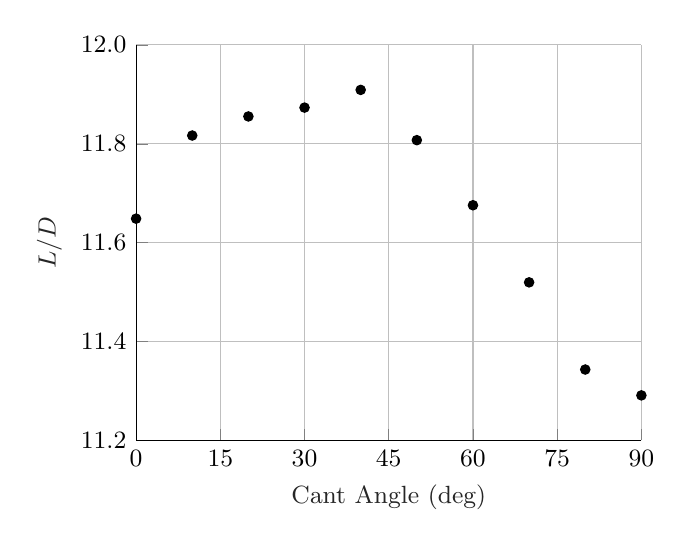
\begin{tikzpicture}

\begin{axis}[%
width=0.969\fwidth,
height=\fheight,
at={(0\fwidth,0\fheight)},
xmin=0,
xmax=90,
xlabel style={font=\color{white!15!black}\small},
xlabel={Cant Angle (deg)},
xtick={0,15,...,90},
ymin=11.2,
ymax=12,
ylabel style={font=\color{white!15!black}\small},
ylabel={$L/D$},
yticklabel style={
            /pgf/number format/fixed,
            /pgf/number format/precision=1,
            /pgf/number format/fixed zerofill
        },
scaled y ticks=false,
axis background/.style={fill=white},
axis x line*=bottom,
axis y line*=left,
xmajorgrids,
ymajorgrids,
tick label style={font=\small}
]
\addplot [color=black, only marks, mark size=1.7pt, mark=*, mark options={solid, black}, forget plot]
  table[row sep=crcr]{%
0	11.64853273\\
10	11.81669992\\
20	11.85528946\\
30	11.87318544\\
40	11.90900866\\
50	11.8073117\\
60	11.67565529\\
70	11.51966778\\
80	11.34330254\\
90	11.29101694\\
};
\end{axis}
\end{tikzpicture}%
    \caption{The lift-to-drag ratio of the airfoil section at various cant angles as calculated by XFLR5.}
    \label{fig:Simu}
\end{figure}


\section{Discussion}

\subsection{Comparison of Experimental Data to XFLR5 Data}

Generally, the experimental data exhibited the expected shape, which included a peak occurring at a cant angle of approximately \ang{40} and a subsequent decrease in the lift-to-drag ratio following this peak.
The increase in the lift-to-drag ratio observed at cant angles below \ang{40} aligned with the theory that the presence of the winglets disrupted the wingtip vortices, resulting in an increase in the lift-to-drag ratio.
Conversely, the decrease observed at high cant angles was consistent with the expectation that, at high cant angles, the increase in skin friction would outweigh the positive effects of implementing winglets in terms of the lift-to-drag ratio.

Another observation is that the experimental data consistently yielded lower lift-to-drag ratios compared to the theoretical XFLR5 data for each cant angle, as illustrated by Fig.~\ref{fig:comp}.
The percentage deviation between the experimental data and the XFLR5 data ranged from 6.4\% to 14.1\%.
This discrepancy was attributed to the surface roughness in the wing caused by the FDM printing process, which created visible ridges in the wing.
The surface roughness contributed to an increase in skin friction, consequently increasing the overall drag force experienced by the wing.
Since the lift-to-drag ratio is inversely proportional to the drag force, this led to an underestimation of the overall lift-to-drag ratio as observed in the experimental data.

\begin{figure}[H]
    \centering
    % This file was created by matlab2tikz.
%
%The latest updates can be retrieved from
%  http://www.mathworks.com/matlabcentral/fileexchange/22022-matlab2tikz-matlab2tikz
%where you can also make suggestions and rate matlab2tikz.
%
\definecolor{mycolor1}{rgb}{0.85000,0.32500,0.09800}%
\definecolor{mycolor2}{rgb}{0.98039,0.27451,0.08627}%
%
\begin{tikzpicture}

\begin{axis}[%
width=0.969\fwidth,
height=\fheight,
at={(0\fwidth,0\fheight)},
xmin=0,
xmax=100,
xlabel style={font=\color{white!15!black}\small},
xlabel={Cant Angle (deg)},
ymin=9,
ymax=13,
ylabel style={font=\color{white!15!black}\small},
ylabel={$L/D$},
axis background/.style={fill=white},
axis x line*=bottom,
axis y line*=left,
xmajorgrids,
ymajorgrids,
tick label style={font=\small},
legend style={legend cell align=left, align=left, draw=white!15!black, font=\small}
]
\addplot [color=black, only marks, mark size=1.7pt, mark=*, mark options={solid, black}]
  table[row sep=crcr]{%
0	11.64853273\\
10	11.81669992\\
20	11.85528946\\
30	11.87318544\\
40	11.90900866\\
50	11.8073117\\
60	11.67565529\\
70	11.51966778\\
80	11.34330254\\
90	11.29101694\\
};
\addlegendentry{XFLR5}

\addplot [color=black, only marks, mark size=2pt, mark=diamond*, mark options={solid, fill=mycolor2, draw=mycolor2}]
plot [error bars/.cd, x dir=both, x explicit, y dir=both, y explicit, error bar style={line width=0.5pt}, error mark options={line width=0.5pt, mark size=3.0pt, rotate=90}]
table[row sep=crcr, y error index=2, x error index=3]{%
0	10.36862817	0.034216472961	1\\
10	10.4378036	0.03444475188	1\\
20	10.44548976	0.034470116208	1\\
30	10.63946302	0.035110227966	1\\
40	10.69422496	0.035290942368	1\\
50	10.62381675	0.035058595275	1\\
60	10.60152292	0.034985025636	1\\
70	10.41259212	0.034361553996	1\\
80	10.390625	0.0342890625	1\\
90	10.07575758	0.033250000014	1\\
};
\addlegendentry{Experimental}

\end{axis}
\end{tikzpicture}%
    \caption{Comparison of experimental lift-to-drag ratios with the theoretical ratios obtained from XFLR5 against varying cant angles.}
    \label{fig:comp}
\end{figure}

\subsection{Characterizing the Cant Angle Relationship}

To determine an equation that would best represent the relationship between the winglet cant angle and the lift-to-drag efficiency ratio of the wing, several different theoretical models were tested to determine which was the most appropriate.
The models considered included a linear, quadratic, cubic, and quartic model.
The suitability of each model was assessed by analyzing the coefficient of determination obtained from performing a regression for each model.
The coefficient of determination is a statistical variable used to evaluate how closely a linear regression matches the observed data~\cite{rSquare}.
For a given data set with dependent values $y$, the coefficient of determination, $R^2$, can be determined using~\eqref{eq:R2}, where $y_i$ denotes an individual data point, $f_i$ is the predicted data point from the model, and $\bar{y}$ is the mean of the data.

\begin{equation} \label{eq:R2}
    R^2 = 1 - \frac{\sum_i \left(y_i - f_i\right)^2}{\sum_i \left(y_i - \bar{y}\right)^2}
\end{equation}

Fig.~\ref{fig:n1}, \ref{fig:n2}, \ref{fig:n3}, and \ref{fig:n4} show the resulting regression models plotted on top of the experimental data.

\begin{figure}[H]
    \centering
    % This file was created by matlab2tikz.
%
%The latest updates can be retrieved from
%  http://www.mathworks.com/matlabcentral/fileexchange/22022-matlab2tikz-matlab2tikz
%where you can also make suggestions and rate matlab2tikz.
%
\definecolor{mycolor1}{rgb}{0.00000,0.44700,0.74100}%
\definecolor{mycolor2}{rgb}{0.98039,0.27451,0.08627}%
%
\begin{tikzpicture}

\begin{axis}[%
width=0.969\fwidth,
height=\fheight,
at={(0\fwidth,0\fheight)},
xmin=0,
xmax=90,
xlabel style={font=\color{white!15!black}\small},
xlabel={Cant Angle (deg)},
xtick={0,15,...,90},
ymin=10,
ymax=10.8,
ylabel style={font=\color{white!15!black}\small},
ylabel={$L/D$},
axis background/.style={fill=white},
axis x line*=bottom,
axis y line*=left,
xmajorgrids,
ymajorgrids,
tick label style={font=\small}
]
\addplot [color=mycolor1, only marks, mark=square*, mark options={solid, fill=mycolor2, draw=mycolor2}, forget plot]
  table[row sep=crcr]{%
0	10.36862817\\
10	10.4378036\\
20	10.44548976\\
30	10.63946302\\
40	10.69422496\\
50	10.62381675\\
60	10.60152292\\
70	10.41259212\\
80	10.390625\\
90	10.07575758\\
};
\addplot [color=black, line width=2.0pt, forget plot]
  table[row sep=crcr]{%
0	10.5593960849091\\
10	10.5393063744848\\
20	10.5192166640606\\
30	10.4991269536364\\
40	10.4790372432121\\
50	10.4589475327879\\
60	10.4388578223636\\
70	10.4187681119394\\
80	10.3986784015152\\
90	10.3785886910909\\
};
\end{axis}
\end{tikzpicture}%
    \caption{Linear fit of the experimental data with $R^2 = 0.11$.}
    \label{fig:n1}
\end{figure}

\begin{figure}[H]
    \centering
    % This file was created by matlab2tikz.
%
%The latest updates can be retrieved from
%  http://www.mathworks.com/matlabcentral/fileexchange/22022-matlab2tikz-matlab2tikz
%where you can also make suggestions and rate matlab2tikz.
%
\definecolor{mycolor1}{rgb}{0.00000,0.44700,0.74100}%
\definecolor{mycolor2}{rgb}{0.98039,0.27451,0.08627}%
%
\begin{tikzpicture}

\begin{axis}[%
width=0.969\fwidth,
height=\fheight,
at={(0\fwidth,0\fheight)},
xmin=0,
xmax=90,
xlabel style={font=\color{white!15!black}\small},
xlabel={Cant Angle (deg)},
xtick={0,15,...,90},
ymin=10,
ymax=10.8,
ylabel style={font=\color{white!15!black}\small},
ylabel={$L/D$},
axis background/.style={fill=white},
axis x line*=bottom,
axis y line*=left,
xmajorgrids,
ymajorgrids,
tick label style={font=\small}
]
\addplot [color=mycolor1, only marks, mark=square*, mark options={solid, fill=mycolor2, draw=mycolor2}, forget plot]
  table[row sep=crcr]{%
0	10.36862817\\
10	10.4378036\\
20	10.44548976\\
30	10.63946302\\
40	10.69422496\\
50	10.62381675\\
60	10.60152292\\
70	10.41259212\\
80	10.390625\\
90	10.07575758\\
};
\addplot [color=black, line width=2.0pt, forget plot]
  table[row sep=crcr]{%
0	10.3080308649091\\
0.909090909090909	10.3231699487824\\
1.81818181818182	10.3379627995702\\
2.72727272727273	10.3524094172727\\
3.63636363636364	10.3665098018898\\
4.54545454545455	10.3802639534215\\
5.45454545454545	10.3936718718678\\
6.36363636363636	10.4067335572287\\
7.27272727272727	10.4194490095041\\
8.18181818181818	10.4318182286942\\
9.09090909090909	10.4438412147989\\
10	10.4555179678182\\
10.9090909090909	10.4668484877521\\
11.8181818181818	10.4778327746006\\
12.7272727272727	10.4884708283636\\
13.6363636363636	10.4987626490413\\
14.5454545454545	10.5087082366336\\
15.4545454545455	10.5183075911405\\
16.3636363636364	10.527560712562\\
17.2727272727273	10.5364676008981\\
18.1818181818182	10.5450282561488\\
19.0909090909091	10.553242678314\\
20	10.5611108673939\\
20.9090909090909	10.5686328233884\\
21.8181818181818	10.5758085462975\\
22.7272727272727	10.5826380361212\\
23.6363636363636	10.5891212928595\\
24.5454545454545	10.5952583165124\\
25.4545454545455	10.6010491070799\\
26.3636363636364	10.606493664562\\
27.2727272727273	10.6115919889587\\
28.1818181818182	10.61634408027\\
29.0909090909091	10.6207499384959\\
30	10.6248095636364\\
30.9090909090909	10.6285229556915\\
31.8181818181818	10.6318901146612\\
32.7272727272727	10.6349110405455\\
33.6363636363636	10.6375857333444\\
34.5454545454545	10.6399141930578\\
35.4545454545455	10.6418964196859\\
36.3636363636364	10.6435324132286\\
37.2727272727273	10.6448221736859\\
38.1818181818182	10.6457657010578\\
39.0909090909091	10.6463629953444\\
40	10.6466140565455\\
40.9090909090909	10.6465188846612\\
41.8181818181818	10.6460774796915\\
42.7272727272727	10.6452898416364\\
43.6363636363636	10.6441559704959\\
44.5454545454545	10.64267586627\\
45.4545454545455	10.6408495289587\\
46.3636363636364	10.638676958562\\
47.2727272727273	10.6361581550799\\
48.1818181818182	10.6332931185124\\
49.0909090909091	10.6300818488595\\
50	10.6265243461212\\
50.9090909090909	10.6226206102975\\
51.8181818181818	10.6183706413884\\
52.7272727272727	10.6137744393939\\
53.6363636363636	10.608832004314\\
54.5454545454545	10.6035433361488\\
55.4545454545455	10.5979084348981\\
56.3636363636364	10.591927300562\\
57.2727272727273	10.5855999331405\\
58.1818181818182	10.5789263326336\\
59.0909090909091	10.5719064990413\\
60	10.5645404323636\\
60.9090909090909	10.5568281326005\\
61.8181818181818	10.5487695997521\\
62.7272727272727	10.5403648338182\\
63.6363636363636	10.5316138347989\\
64.5454545454545	10.5225166026942\\
65.4545454545455	10.5130731375041\\
66.3636363636364	10.5032834392286\\
67.2727272727273	10.4931475078678\\
68.1818181818182	10.4826653434215\\
69.0909090909091	10.4718369458898\\
70	10.4606623152727\\
70.9090909090909	10.4491414515702\\
71.8181818181818	10.4372743547824\\
72.7272727272727	10.4250610249091\\
73.6363636363636	10.4125014619504\\
74.5454545454545	10.3995956659063\\
75.4545454545455	10.3863436367769\\
76.3636363636364	10.372745374562\\
77.2727272727273	10.3588008792617\\
78.1818181818182	10.344510150876\\
79.0909090909091	10.329873189405\\
80	10.3148899948485\\
80.9090909090909	10.2995605672066\\
81.8181818181818	10.2838849064793\\
82.7272727272727	10.2678630126667\\
83.6363636363636	10.2514948857686\\
84.5454545454545	10.2347805257851\\
85.4545454545455	10.2177199327163\\
86.3636363636364	10.200313106562\\
87.2727272727273	10.1825600473223\\
88.1818181818182	10.1644607549972\\
89.0909090909091	10.1460152295868\\
90	10.1272234710909\\
};
\end{axis}
\end{tikzpicture}%
    \caption{Quadratic fit of the experimental data with $R^2 = 0.89$.}
    \label{fig:n2}
\end{figure}

\begin{figure}[H]
    \centering
    % This file was created by matlab2tikz.
%
%The latest updates can be retrieved from
%  http://www.mathworks.com/matlabcentral/fileexchange/22022-matlab2tikz-matlab2tikz
%where you can also make suggestions and rate matlab2tikz.
%
\definecolor{mycolor1}{rgb}{0.00000,0.44700,0.74100}%
\definecolor{mycolor2}{rgb}{0.98039,0.27451,0.08627}%
%
\begin{tikzpicture}

\begin{axis}[%
width=0.969\fwidth,
height=\fheight,
at={(0\fwidth,0\fheight)},
xmin=0,
xmax=90,
xlabel style={font=\color{white!15!black}\small},
xlabel={Cant Angle (deg)},
xtick={0,15,...,90},
ymin=10,
ymax=10.8,
ylabel style={font=\color{white!15!black}\small},
ylabel={$L/D$},
axis background/.style={fill=white},
axis x line*=bottom,
axis y line*=left,
xmajorgrids,
ymajorgrids,
tick label style={font=\small}
]
\addplot [color=mycolor1, only marks, mark=square*, mark options={solid, fill=mycolor2, draw=mycolor2}, forget plot]
  table[row sep=crcr]{%
0	10.36862817\\
10	10.4378036\\
20	10.44548976\\
30	10.63946302\\
40	10.69422496\\
50	10.62381675\\
60	10.60152292\\
70	10.41259212\\
80	10.390625\\
90	10.07575758\\
};
\addplot [color=black, line width=2.0pt, forget plot]
  table[row sep=crcr]{%
0	10.3494806813566\\
0.909090909090909	10.3579086942724\\
1.81818181818182	10.3663500884453\\
2.72727272727273	10.3747974491467\\
3.63636363636364	10.3832433616477\\
4.54545454545455	10.3916804112198\\
5.45454545454545	10.4001011831342\\
6.36363636363636	10.4084982626622\\
7.27272727272727	10.416864235075\\
8.18181818181818	10.425191685644\\
9.09090909090909	10.4334731996405\\
10	10.4417013623357\\
10.9090909090909	10.4498687590009\\
11.8181818181818	10.4579679749074\\
12.7272727272727	10.4659915953265\\
13.6363636363636	10.4739322055295\\
14.5454545454545	10.4817823907877\\
15.4545454545455	10.4895347363724\\
16.3636363636364	10.4971818275548\\
17.2727272727273	10.5047162496062\\
18.1818181818182	10.512130587798\\
19.0909090909091	10.5194174274014\\
20	10.5265693536876\\
20.9090909090909	10.5335789519281\\
21.8181818181818	10.5404388073941\\
22.7272727272727	10.5471415053568\\
23.6363636363636	10.5536796310875\\
24.5454545454545	10.5600457698576\\
25.4545454545455	10.5662325069384\\
26.3636363636364	10.572232427601\\
27.2727272727273	10.5780381171169\\
28.1818181818182	10.5836421607572\\
29.0909090909091	10.5890371437933\\
30	10.5942156514965\\
30.9090909090909	10.599170269138\\
31.8181818181818	10.6038935819892\\
32.7272727272727	10.6083781753213\\
33.6363636363636	10.6126166344056\\
34.5454545454545	10.6166015445135\\
35.4545454545455	10.6203254909161\\
36.3636363636364	10.6237810588848\\
37.2727272727273	10.6269608336909\\
38.1818181818182	10.6298574006056\\
39.0909090909091	10.6324633449003\\
40	10.6347712518462\\
40.9090909090909	10.6367737067146\\
41.8181818181818	10.6384632947768\\
42.7272727272727	10.6398326013041\\
43.6363636363636	10.6408742115678\\
44.5454545454545	10.6415807108392\\
45.4545454545455	10.6419446843895\\
46.3636363636364	10.6419587174901\\
47.2727272727273	10.6416153954121\\
48.1818181818182	10.6409073034271\\
49.0909090909091	10.6398270268061\\
50	10.6383671508205\\
50.9090909090909	10.6365202607416\\
51.8181818181818	10.6342789418407\\
52.7272727272727	10.631635779389\\
53.6363636363636	10.6285833586579\\
54.5454545454545	10.6251142649186\\
55.4545454545455	10.6212210834424\\
56.3636363636364	10.6168963995007\\
57.2727272727273	10.6121327983646\\
58.1818181818182	10.6069228653055\\
59.0909090909091	10.6012591855947\\
60	10.5951343445035\\
60.9090909090909	10.5885409273031\\
61.8181818181818	10.5814715192648\\
62.7272727272727	10.57391870566\\
63.6363636363636	10.5658750717599\\
64.5454545454545	10.5573332028357\\
65.4545454545455	10.5482856841589\\
66.3636363636364	10.5387251010006\\
67.2727272727273	10.5286440386322\\
68.1818181818182	10.5180350823249\\
69.0909090909091	10.5068908173501\\
70	10.495203828979\\
70.9090909090909	10.4829667024829\\
71.8181818181818	10.4701720231331\\
72.7272727272727	10.4568123762009\\
73.6363636363636	10.4428803469576\\
74.5454545454545	10.4283685206745\\
75.4545454545455	10.4132694826227\\
76.3636363636364	10.3975758180738\\
77.2727272727273	10.3812801122988\\
78.1818181818182	10.3643749505692\\
79.0909090909091	10.3468529181561\\
80	10.328706600331\\
80.9090909090909	10.309928582365\\
81.8181818181818	10.2905114495295\\
82.7272727272727	10.2704477870958\\
83.6363636363636	10.2497301803351\\
84.5454545454545	10.2283512145187\\
85.4545454545455	10.2063034749179\\
86.3636363636364	10.183579546804\\
87.2727272727273	10.1601720154484\\
88.1818181818182	10.1360734661222\\
89.0909090909091	10.1112764840967\\
90	10.0857736546434\\
};
\end{axis}
\end{tikzpicture}%
    \caption{Cubic fit of the experimental data with $R^2 = 0.92$.}
    \label{fig:n3}
\end{figure}

\begin{figure}[H]
    \centering
    % This file was created by matlab2tikz.
%
%The latest updates can be retrieved from
%  http://www.mathworks.com/matlabcentral/fileexchange/22022-matlab2tikz-matlab2tikz
%where you can also make suggestions and rate matlab2tikz.
%
\definecolor{mycolor1}{rgb}{0.00000,0.44700,0.74100}%
\definecolor{mycolor2}{rgb}{0.98039,0.27451,0.08627}%
%
\begin{tikzpicture}

\begin{axis}[%
width=0.969\fwidth,
height=0.9\fheight,
at={(0\fwidth,0\fheight)},
xmin=0,
xmax=90,
xlabel style={font=\color{white!15!black}\small},
xlabel={Cant Angle (deg)},
xtick={0,15,...,90},
ymin=10,
ymax=10.8,
ylabel style={font=\color{white!15!black}\small},
ylabel={$L/D$},
axis background/.style={fill=white},
axis x line*=bottom,
axis y line*=left,
xmajorgrids,
ymajorgrids,
tick label style={font=\small}
]
\addplot [color=mycolor1, only marks, mark=square*, mark options={solid, fill=mycolor2, draw=mycolor2}, forget plot]
  table[row sep=crcr]{%
0	10.36862817\\
10	10.4378036\\
20	10.44548976\\
30	10.63946302\\
40	10.69422496\\
50	10.62381675\\
60	10.60152292\\
70	10.41259212\\
80	10.390625\\
90	10.07575758\\
};
\addplot [color=black, line width=2.0pt, forget plot]
  table[row sep=crcr]{%
0	10.3660572397203\\
0.909090909090909	10.3685213826012\\
1.81818181818182	10.3716087229074\\
2.72727272727273	10.3752816538772\\
3.63636363636364	10.3795031977495\\
4.54545454545455	10.3842370057638\\
5.45454545454545	10.3894473581604\\
6.36363636363636	10.3950991641802\\
7.27272727272727	10.401157962065\\
8.18181818181818	10.407589919057\\
9.09090909090909	10.4143618313993\\
10	10.4214411243357\\
10.9090909090909	10.4287958521104\\
11.8181818181818	10.4363946979687\\
12.7272727272727	10.4442069741562\\
13.6363636363636	10.4522026219195\\
14.5454545454545	10.4603522115058\\
15.4545454545455	10.4686269421628\\
16.3636363636364	10.4769986421392\\
17.2727272727273	10.4854397686842\\
18.1818181818182	10.4939234080476\\
19.0909090909091	10.5024232754802\\
20	10.5109137152331\\
20.9090909090909	10.5193697005584\\
21.8181818181818	10.5277668337088\\
22.7272727272727	10.5360813459377\\
23.6363636363636	10.544290097499\\
24.5454545454545	10.5523705776476\\
25.4545454545455	10.5603009046389\\
26.3636363636364	10.5680598257289\\
27.2727272727273	10.5756267171746\\
28.1818181818182	10.5829815842334\\
29.0909090909091	10.5901050611635\\
30	10.5969784112238\\
30.9090909090909	10.6035835266738\\
31.8181818181818	10.6099029287739\\
32.7272727272727	10.615919767785\\
33.6363636363636	10.6216178229686\\
34.5454545454545	10.6269815025872\\
35.4545454545455	10.6319958439038\\
36.3636363636364	10.636646513182\\
37.2727272727273	10.6409198056863\\
38.1818181818182	10.6448026456817\\
39.0909090909091	10.6482825864341\\
40	10.6513478102098\\
40.9090909090909	10.653987128276\\
41.8181818181818	10.6561899809007\\
42.7272727272727	10.6579464373522\\
43.6363636363636	10.6592471958999\\
44.5454545454545	10.6600835838135\\
45.4545454545455	10.6604475573639\\
46.3636363636364	10.6603317018221\\
47.2727272727273	10.6597292314602\\
48.1818181818182	10.6586339895509\\
49.0909090909091	10.6570404483676\\
50	10.6549437091841\\
50.9090909090909	10.6523395022754\\
51.8181818181818	10.6492241869168\\
52.7272727272727	10.6455947513845\\
53.6363636363636	10.6414488129551\\
54.5454545454545	10.6367846179063\\
55.4545454545455	10.6316010415162\\
56.3636363636364	10.6258975880637\\
57.2727272727273	10.6196743908283\\
58.1818181818182	10.6129322120902\\
59.0909090909091	10.6056724431305\\
60	10.5978971042308\\
60.9090909090909	10.5896088446733\\
61.8181818181818	10.580810942741\\
62.7272727272727	10.5715073057177\\
63.6363636363636	10.5617024698878\\
64.5454545454545	10.5514016005362\\
65.4545454545455	10.5406104919489\\
66.3636363636364	10.5293355674121\\
67.2727272727273	10.5175838792131\\
68.1818181818182	10.5053631086397\\
69.0909090909091	10.4926815659804\\
70	10.4795481905245\\
70.9090909090909	10.4659725505617\\
71.8181818181818	10.4519648433828\\
72.7272727272727	10.4375358952789\\
73.6363636363636	10.422697161542\\
74.5454545454545	10.4074607264649\\
75.4545454545455	10.3918393033408\\
76.3636363636364	10.3758462344637\\
77.2727272727273	10.3594954911285\\
78.1818181818182	10.3428016736304\\
79.0909090909091	10.3257800112657\\
80	10.308446362331\\
80.9090909090909	10.2908172141239\\
81.8181818181818	10.2729096829425\\
82.7272727272727	10.2547415140857\\
83.6363636363636	10.2363310818531\\
84.5454545454545	10.2176973895448\\
85.4545454545455	10.1988600694619\\
86.3636363636364	10.1798393829058\\
87.2727272727273	10.1606562201789\\
88.1818181818182	10.1413321005843\\
89.0909090909091	10.1218891724255\\
90	10.102350213007\\
};
\end{axis}
\end{tikzpicture}%
    \caption{Quartic fit of the experimental data with $R^2 = 0.93$.}
    \label{fig:n4}
\end{figure}
\noindent
The $R^2$ values for the four models are summarized in Table~\ref{tab:models}.

\begin{table}[H]
    \centering
    \caption{Coefficient of Determination for Each Model}
    \renewcommand{\arraystretch}{1.1}
    \begin{tabular}{cc}
    \toprule
    Model & Coefficient of Determination, $R^2$ \\ \midrule \midrule
    Linear & 0.11 \\
    Quadratic & 0.89 \\
    Cubic & 0.92 \\
    Quartic & 0.93 \\ \bottomrule
    \end{tabular}
    \label{tab:models}
\end{table}

From Table~\ref{tab:models}, the quartic model was the most accurate in fitting the experimental data, followed by the cubic model.
This finding is consistent with the visual analysis of Fig.~\ref{fig:n3} and \ref{fig:n4}, where both models appear to closely match the experimental data.
The regression for the quartic model resulted in~\eqref{eq:quartic} for the best fit polynomial, where ${L/D}_\text{quartic}$ is the predicted lift-to-drag ratio from the quartic model, and $\Gamma$ is the cant angle.

\begin{equation} \label{eq:quartic}
    \begin{split}
        {L/D}_\text{quartic} &= (\num{4.0e-8})\Gamma^4 - (\num{9.0e-6})\Gamma^3 \\
        &\quad + (\num{4.0e-4})\Gamma^2 + (\num{2.4e-3})\Gamma + 10.37
    \end{split}
\end{equation}

\subsection{Determining the Optimal Winglet Cant Angle}

To determine the theoretical optimal winglet cant angle, the local maximum of the quartic model was found.
This was achieved by taking the derivative of the quartic model with respect to $\Gamma$, as shown in~\eqref{eq:derivative}.
\begin{equation} \label{eq:derivative}
    \begin{split}
        \frac{d{L/D}_\text{quartic}}{d\Gamma} &= (\num{1.6e-7})\Gamma^3 - (\num{2.7e-5})\Gamma^2 \\
        &\quad + (\num{8.0e-4})\Gamma + \num{2.4e-3}
    \end{split}
\end{equation}
A local extremum occurs when the first derivative is equal to zero.
Setting~\eqref{eq:derivative} equal to zero and solving for the roots of $\Gamma$ yields solutions at \ang{-2.74}, \ang{42.36}, and \ang{129.13}.
Considering the bounds $\ang{0} \leq \Gamma \leq \ang{90}$ from the experimental data, the local maximum occurs at $42 \pm \ang{1}$.
The model exhibits a maximum percent error of 2.3\% when compared to the experimental data.
This error is associated with the \ang{80} cant angle.
The fact that the percent error generally increased for higher cant angles indicates that high cant angle winglets may make the flow more turbulent, causing variability in the aerodynamic forces.


\section{Conclusion}


Ultimately, it was found that the effect of winglet cant angle on the lift-to-drag ratio followed a quartic trend, with a peak occurring at an angle of about \ang{40}.
The increase in the lift-to-drag ratio before this peak is due to the winglets disrupting the formation of wingtip vortices, which reduces the induced drag.
However, if the cant angle is increased beyond this peak, it results in additional skin friction and a decrease in the lift-to-drag ratio.

When comparing the experimental data to theoretical data obtained from XFLR5, it was observed that the shapes of both plots are similar, as shown in Fig.~\ref{fig:comp}.
However, the lift-to-drag ratios for the experimental data were consistently lower than those of the theoretical data.
This is likely due to the presence of ridges on the surface of the wing from the 3D printing process.
The increase in surface roughness caused by these ridges increased the total drag force acting on the wing.
Using a different 3D printing method such as stereolithography would reduce the prominence of these ridges and would yield drag forces closer to the theoretical data.

Additionally, the method of mounting the wing to the dynamometer could be improved.
In this experiment, tape was required to restrict the movement of the wing section, preventing it from spinning.
To improve this, the orientation of the screw can be adjusted so that when fully threaded, the wing is in the correct orientation.
This will eliminate any additional drag introduced by the tape.

To further expand on the results of the experiment, the tips of the airfoil can be modified so that they transition from an airfoil cross-section to a closed edge.
This can be done by tapering the edge of the airfoil section until it forms a sharp edge.
This modification will decrease the parasitic drag generated by the wingtip, thus increasing efficiency impact that the wingtip has on the wing and making any efficiency gains more pronounced.


\section*{Appendix A: Uncertainty Calculations}


\begin{table}[H]
    \renewcommand{\arraystretch}{1.35}
    \centering
    \caption{Summary of Measurement Uncertainties}
    \begin{tabular}{cccc}
    \toprule
    Parameter & Symbol & Justification & Uncertainty ($\pm$) \\ \midrule \midrule
    Temperature & $\mu T$ & Digital & \qty{0.1}{\celsius} \\
    Humidity & $\mu \varphi$ & Digital & 1\% \\
    Ambient Pressure & $\mu P_\text{amb}$ & Barometer & \qty{0.02}{mm\ce{Hg}} \\
    \makecell{Static Pressure \\ Difference} & $\mu \Delta P$ & \makecell{95\% Conf. \\ Int.} & \qty{0.55}{\Pa} \\
    Saturation Pressure & $\mu P_g$ & RSS & \qty{15.22}{\pascal} \\
    Density & $\mu \rho$ & RSS & \qty{0.004}{\kg\per\m\cubed} \\
    Airfoil Chord Length & $\mu c$ & Calipers & \qty{0.2}{\mm} \\
    \makecell{Tunnel Calibration \\ Coefficient} & $\mu K$ & \cite{lab1} & 0.002 \\
    Kinematic Viscosity & $\mu \nu$ & \cite{HeatTrans} & \qty{2e-9}{\m\squared\per\s} \\
    Reynolds Number & $\mu Re$ & RSS & 184.4 \\
    Lift & $\mu L$ & Max. \% Error & 0.81\% \\
    Drag & $\mu D$ & Max. \% Error & 0.94\% \\
    Lift-to-drag Ratio & $\mu L/D$ & RSS & Variable \\
    Cant Angle & $\mu \Gamma$ & \cite{3Dangle} & \ang{1} \\
    Voltage & $\mu V$ & \cite{Transduce} & 0.05\% of voltage \\ \bottomrule
    \end{tabular}
    \label{tab:uncertainty}
\end{table}

The uncertainties for each measured value are summarized in Table~\ref{tab:uncertainty}.
First, the systemic bias in the reading of the transducer static pressure readings was accounted for by zeroing the pressure value in the LabVIEW VI.
The random uncertainty for each static pressure reading was then obtained by using a 95\% confidence interval with a normal distribution.
Because a sample size of 4000 was used for each reading, it was determined to be sufficiently large that the sample distribution approached the normal distribution according to the central limit theorem~\cite{MoMLecture}.
A $z^*$ value of 1.96 was used for the calculation of the 95\% confidence interval.
The margin of error then served as the uncertainty, as seen in~\eqref{eq:conf}, where $\mu X$ is the margin of error for an arbitrary measurement, $S_x$ is the sample standard deviation, and $n$ is the number of samples~\cite{MoMLecture}.

\begin{equation} \label{eq:conf}
    \mu X = z^* \frac{S_x}{\sqrt{n}}
\end{equation}

The uncertainty in the saturation pressure, $P_g$, was calculated using error propagation theory, as shown by~\eqref{eq:uPsat}, where $T$ is the ambient temperature~\cite{errorprop}.

\begin{equation} \label{eq:uPsat}
    \mu P_g = \mu T \frac{\partial P_g}{\partial T}
\end{equation}

The uncertainty in the fluid density, $\rho$, was calculated using the RSS method, as shown by~\eqref{eq:uRho}, where $P$ is the ambient pressure, $T$ is the ambient temperature, $\varphi$ is the relative humidity, and $P_g$ is the saturation pressure.

\begin{equation} \label{eq:uRho}
    \resizebox{227pt}{!}{$\displaystyle{\mu \rho = \left[\left(\mu P \frac{\partial \rho}{\partial P}\right)^2 + \left(\mu T \frac{\partial \rho}{\partial T}\right)^2 + \left(\mu \varphi \frac{\partial \rho}{\partial \varphi}\right)^2 + \left(\mu P_g \frac{\partial \rho}{\partial P_g}\right)^2\right]^{1/2}}$}
\end{equation}

The uncertainty in the Reynolds number, $Re$, was calculated using the RSS method, as shown by~\eqref{eq:uRe}, where $\Delta P$ is the static pressure difference, $\nu$ is the dynamic viscosity of the fluid, $\rho$ is the density of the fluid, and $c$ is the chord length of the airfoil.

\begin{equation} \label{eq:uRe}
    \resizebox{227pt}{!}{$\displaystyle{\mu Re = \left[\left(\mu \Delta P \frac{\partial Re}{\partial \Delta P}\right)^2 + \left(\mu \nu \frac{\partial Re}{\partial \nu}\right)^2 + \left(\mu \rho \frac{\partial Re}{\partial \rho}\right)^2 + \left(\mu c \frac{\partial Re}{\partial c}\right)^2\right]^{1/2}}$}
\end{equation}

The uncertainties in the lift and drag values obtained from the dynamometer were determined by calculating the maximum percent error deviation from the calibration curve.
As an example, Fig.~\ref{fig:calL} displays the calibration data, as well as the line of best fit that relates the voltage data to the weight. 

The percentage error between the actual calibration data and the line of best fit was calculated for each voltage point.
It was determined that the line of best fit had a maximum percent error of 0.81\% at worst.
Therefore, it was assumed that the interpolated lift values obtained from the voltage measurements from the dynamometer would have a percent error of 0.81\%.
This uncertainty was applied to all the lift values in the experiment.
A similar process was also conducted for the drag values.

\pagebreak
The uncertainty in the lift-to-drag ratio, $L/D$, was calculated using the RSS method, as shown by~\eqref{eq:uLD}, where $L$ is the interpolated lift force, and $D$ is the interpolated drag force.

\begin{equation} \label{eq:uLD}
    \mu L/D = \left[\left(\mu L \frac{\partial L/D}{\partial L}\right)^2 + \left(\mu D \frac{\partial L/D}{\partial D}\right)^2\right]^{1/2}
\end{equation}

This lab report was typeset using \LaTeX.

\begin{thebibliography}{99}
    \bibitem{FAA} Federal Aviation Administration, ``Air Traffic By The Numbers,'' URL: \url{https://www.faa.gov/air_traffic/by_the_numbers}, Apr 2023.
    \bibitem{NASA} Hall, N., ``Winglets,'' \textit{National Aeronautics and Space Administration}, URL: \url{https://www1.grc.nasa.gov/beginners-guide-to-aeronautics/winglets/}, 2023.
    \bibitem{cantDiag} Myilsamy, D., Thirumalai, Y., and Premkumar, P. S., ``Performance Investigation of an Aircraft Wing at Various Cant Angles of Winglets using CFD Simulation,'' \textit{Altair Technology Conference 2015}, Banglore, India, 2015.
    \bibitem{variableCant} Swargam, L., Kidron, M., Nandigam, M. L., and Dwivedi, Y. D., ``Effect of Variable Cant Angle on Sweepback Wing,'' \textit{Reviews on Modern Technologies for Aircraft and Aero-Engines}, Vol. 1, No. 9, Apr 2022, pp. 61--68.
    \bibitem{lab1} Borg., A., Lam., B., Latzko, A., ``Wind Tunnel Calibration for Prediction of Testing Conditions,'' \textit{University of Florida}, 2023.
    \bibitem{rSquare} Glantz, S. A., Slinker, B. K., and Neilands, T. B., ``Selecting the `Best' Regression Model,'' \textit{Primer of Applied Regression and Analysis of Variance}, McGraw-Hill, New York, 2016, pp. 335--380.
    \bibitem{HeatTrans} Bergman, T. L., and Lavine, A. S., ``Appendix A: Thermophysical Properties of Matter,'' \textit{Fundamentals of Heat and Mass Transfer}, Wiley, Hoboken, NJ, 2017, p. 911.
    \bibitem{3Dangle} Markforged, ``How to Create High Quality STL Files for 3D Prints,'' URL: \url{https://markforged.com/resources/blog/how-to-create-high-quality-stl-files-for-3d-prints}.
    \bibitem{Transduce} Schaevitz Sensors HR Series Data Sheet, Measurement Specialties, Inc., Hampton, VA, 2015.
    \bibitem{MoMLecture} Ridgeway, S., ``MOM\_lab Uncertainty basics w tension,'' \textit{University of Florida} [PowerPoint slides], URL: \url{https://ufl.instructure.com/courses/447927/files/65674680}, 2022.
    \bibitem{errorprop} Ku, H. H., ``Notes on the Use of Propagation of Error Formulas'', \textit{Journal of Research of the National Bureau of Standards}, Vol. 70C, No. 4, 27 May 1966, pp. 263--273.
\end{thebibliography}

\end{document}